%%%%%%%%%%%%%%%%%%%%%%% file template.tex %%%%%%%%%%%%%%%%%%%%%%%%%
%
% This is a general template file for the LaTeX package SVJour3
% for Springer journals.          Springer Heidelberg 2010/09/16
%
% Copy it to a new file with a new name and use it as the basis
% for your article. Delete % signs as needed.
%
% This template includes a few options for different layouts and
% content for various journals. Please consult a previous issue of
% your journal as needed.
%
%%%%%%%%%%%%%%%%%%%%%%%%%%%%%%%%%%%%%%%%%%%%%%%%%%%%%%%%%%%%%%%%%%%
%
% First comes an example EPS file -- just ignore it and
% proceed on the \documentclass line
% your LaTeX will extract the file if required
\begin{filecontents*}{example.eps}
%!PS-Adobe-3.0 EPSF-3.0
%%BoundingBox: 19 19 221 221
%%CreationDate: Mon Sep 29 1997
%%Creator: programmed by hand (JK)
%%EndComments
gsave
newpath
  20 20 moveto
  20 220 lineto
  220 220 lineto
  220 20 lineto
closepath
2 setlinewidth
gsave
  .4 setgray fill
grestore
stroke
grestore
\end{filecontents*}
%
\RequirePackage{fix-cm}
%
%\documentclass{svjour3}                     % onecolumn (standard format)
%\documentclass[smallcondensed]{svjour3}     % onecolumn (ditto)
\documentclass[smallextended]{svjour3}       % onecolumn (second format)
%\documentclass[twocolumn]{svjour3}          % twocolumn
%
\usepackage{amsmath,amssymb}
\usepackage{framed}
\usepackage{enumitem}
\setlist[enumerate]{leftmargin=*}
\usepackage{comment}
\usepackage[noresetcount,lined,boxed,linesnumbered]{algorithm2e}

\smartqed  % flush right qed marks, e.g. at end of proof
%
\usepackage{graphicx}
\usepackage{natbib}
\bibpunct[, ]{(}{)}{,}{a}{}{,}%
\def\bibfont{\small}%
\def\bibsep{\smallskipamount}%
\def\bibhang{24pt}%
\def\newblock{\ }%
\def\BIBand{and}%

\usepackage{endnotes}
\let\footnote=\endnote
\let\enotesize=\normalsize
\def\notesname{Endnotes}%
\def\makeenmark{$^{\theenmark}$}
\def\enoteformat{\rightskip0pt\leftskip0pt\parindent=1.75em
	\leavevmode\llap{\theenmark.\enskip}}

\renewcommand{\arraystretch}{1.2}
%
% \usepackage{mathptmx}      % use Times fonts if available on your TeX system
%
% insert here the call for the packages your document requires
%\usepackage{latexsym}
% etc.
%
% please place your own definitions here and don't use \def but
% \newcommand{}{}
%
% Insert the name of "your journal" with
% \journalname{myjournal}
%

\newcommand{\supe}{\mathop{\hbox{\rm sup}}}
\newcommand{\maximize}[1]{\displaystyle\maxim_{#1}}
\newcommand{\maxim}{\mathop{\hbox{\rm maximize}}}
\newcommand{\maximi}[1]{\displaystyle\maxi_{#1}}
\newcommand{\maxi}{\mathop{\hbox{\rm max}}}
\newcommand{\minimize}[1]{\displaystyle\minim_{#1}}
\newcommand{\minim}{\mathop{\hbox{\rm minimize}}}
\newcommand{\minimi}[1]{\displaystyle\mini_{#1}}
\newcommand{\mini}{\mathop{\hbox{\rm min}}}
\newcommand{\amin}{\mathop{\mbox{argmin}}}
\newcommand{\amax}{\mathop{\mbox{argmax}}}
\newcommand{\st}{\mathrm{subject\ to}}
\newcommand{\Cal}{\mathcal}
\newcommand{\norm}[1]{\left\Vert#1\right\Vert}
\newcommand{\abs}[1]{\left\vert#1\right\vert}
\newcommand{\set}[1]{\left\{#1\right\}}
\newcommand{\Real}{\mathbb R}
\newcommand{\where}{\mathrm{where}}
\newcommand{\Hif}{{H}_{i, f}}
\newcommand{\N}{\mathcal{N}}
\newcommand{\J}{\mathcal{J}}
\newcommand{\E}{\mathbb{E}}
\newcommand{\D}{\mathbb{D}}
\newcommand{\free}{\mathrm{free}}
\newcommand{\1}{\mathbf{1}}
\newcommand{\indicator}[1]{\mathbbm{1}_{\left[ {#1} \right] }}      
\newcommand{\dps}{\displaystyle}
\newcommand{\ubar}[1]{\text{\b{$#1$}}}

\begin{document}

\title{Equilibrium Wind Hedge Contract Structures Through Nash Bargaining%\thanks{Grants or other notes
%about the article that should go on the front page should be
%placed here. General acknowledgments should be placed at the end of the article.}
}
%\subtitle{Do you have a subtitle?\\ If so, write it here}

%\titlerunning{Short form of title}        % if too long for running head

\author{First Author         \and
        Second Author %etc.
}

%\authorrunning{Short form of author list} % if too long for running head

\institute{F. Author \at
              first address \\
              Tel.: +123-45-678910\\
              Fax: +123-45-678910\\
              \email{fauthor@example.com}           %  \\
%             \emph{Present address:} of F. Author  %  if needed
           \and
           S. Author \at
              second address
}

\date{Received: date / Accepted: date}
% The correct dates will be entered by the editor


\maketitle

\begin{abstract}
With the continued maturing of electricity markets, merchant wind project developers are increasingly looking to long-term hedge contracts to control their exposure to market risks as well as to secure project financing.  Such contracts are usually negotiated with load serving entities looking to hedge against spot price volatility or financial firms who repackage the electricity through structured deals that create value. We model the negotiation process using the Nash bargaining framework. The equilibrium price and quantity come out as the optimal solutions of a stochastic program wherein the objective is to maximize the product of the utility differentials for the two parties, with and without the contract. We use conditional cash flow at risk, a risk based profitability measure, to capture the risk attitudes of the bargaining parties. After incorporating the risk measure into the utility functions, we solve the resulting stochastic program using the sample average approximation method. We present numerical results as well as sensitivity analysis for the equilibrium contract structure with respect to volatility and correlation between a wind plant's outputs and spot electricity prices. We also study how the risk attitudes of the two parties affect the equilibrium structure.
\keywords{wind hedge, Nash bargaining, sample average approximation, global optimization}
% \PACS{PACS code1 \and PACS code2 \and more}
% \subclass{MSC code1 \and MSC code2 \and more}
\end{abstract}

\section{Introduction and Background}

how does this works 

\noindent Growing economic and social pressures in recent times have contributed to the prominence of renewable energy sources as an alternative to conventional electricity production. The last decade has seen a significant increase in wind energy production, especially in developed nations. One of the key advantages of wind power is that it is essentially free of fuel costs and air pollutant emissions. Therefore generating wind power generally has low operating costs. However wind power projects are capital intensive, which makes risk management a key issue. Wind energy producers have to deal with the inherent uncertainties present in the generation capacities as a result of variation in wind-speed as well as the financial risk caused by electricity spot price volatility. To obtain sufficient capital financing for projects, producers are often required to enter into long-term contracts with credit-worthy power purchasers for the purpose of out-sourcing the risk.\\

\noindent The contracts may take the form of long-term power purchase agreements in which the wind farm sells a fixed quantity to an electricity retailer at a fixed price over a certain period of time. Such contracts involve physical delivery of electricity which may be complicated by the transmission process. The wind farm may also resort to purely financial Contract-for-Difference (CFD) hedges in which the two counterparties agree to a fixed quantity, strike price and maturity period. Once the spot-market price of electricity is known the parties settle the difference between the strike price and the spot price amongst themselves. Either type of contract may include the sale of Renewable Energy Certificates (RECs) as well. Since there is no actual transfer of electricity involved in a CFD hedge, such contracts may be entered into not just with electricity retailers but also other parties such as investment firms.\\

\noindent The viability of such long-term hedging contracts hinges on the difference in risk-aversion between the wind power producer and the power purchaser. In this context it becomes important for both parties to analyze the risk-return implications of the contract so as to arrive at optimal contract parameters that maximizes return while restricting the risk involved to acceptable levels.\\

\noindent Although the problem of risk management in the context of electricity derivatives has received some attention, not much work has been done in the bargaining and negotiation framework. An iterative negotiation scheme for bilateral electricity contracts, which enables the counter parties to reach mutually beneficial and risk tolerable contract payoffs was proposed in \cite{4162589}. Nash bargaining theory was used in \cite{dong_equilibrium_2007} to derive contract structures for nonstorable commodities. However the focus there was on a mean-variance based risk analysis, which has severe limitations as we shall explain. A similar model for studying forward contract negotiations in the electricity market was used in \cite{RePEc:isu:genres:32005}, where cross market effects were analyzed. \\

\noindent In this paper, we analyze the risk management aspect of a long term CFD contract between the wind farm and a buyer. We model the negotiation process as a Nash Bargaining game \cite{nash_bargaining_1950}. We model the risk preferences of the two parties using the Conditional Cash Flow at Risk (CCFaR) risk measure \cite{rockafellar_optimization_2000, prokopczuk_quantifying_2007}. The equilibrium solution to the bargaining game is characterized by a stochastic optimization problem which we solve using the sample average approximation (SAA) method \cite{kleywegt_sample_2002, shapiro_lectures_2009}.\\

\noindent The remainder of the paper is organized as follows. Section 2 describes the model we use for the negotiation process and gives a brief review of the utility functions we use. The formulation of the Nash bargaining optimization problem is given in Section 3 along with certain reformulations to make the problem more tractable. An algorithm based on the SAA method is given in Section 4. Some preliminary computational experiences are given in Section 5 and the study is concluded in Section 6 along with planned future extensions of this work.\\


\section{Contract Model}
\label{S:contract-model}

\noindent The transaction we study is a Contract-For-Differences (CFD) between a wind farm and a counter-party such as a load serving entity or a power marketer. The wind farm will hence forth be referred to as the seller and the counter-party will be referred to as the buyer. The two parties negotiate a contract structure, which involves agreement upon a maturity period, strike price and quantity as well as the settlement mechanism and frequency. Settlements are usually paid out every month. Each month, if the average spot price is above the agreed upon strike price, then the wind farm compensates the buyer for the difference. Conversely, if the average spot price is below the strike price, then the buyer will pay the difference to the wind farm. The data and parameters associated with the model are given below in Tables~\ref{inputdata} and \ref{var_funs}.\\

\vspace*{-1pt}
\begin{table}[htp] 
	\caption{Input Data}
	\label{inputdata}
	\begin{tabular}{ll}
		$T$          &The maturity period of a hedge contract, in months.\\
		$\omega$   & Random variable defined on a probability space $(\Omega, \mathcal{F}, P)$ of the underlying uncertainties.\\
		$K_t(\omega)$ &  Capacity of a wind power plant at time $t$ with $t\leq T$; [MW]. \\
		$p_t(\omega)$ &  Wholesale electricity price at time $t$ with $t\leq T$; [\$/MWh]. \\
		$r$  & Risk-free discount rate. \\
		$\delta_t$ & Discount factor at time $t$; $\delta_t = 1/(1 + r)^t$. \\
		$\lambda^B$, $\kappa^B$ & Measures of the buyer's risk aversion. \\
		$\lambda^S$, $\kappa^S$ & Measures of the seller's risk aversion.
	\end{tabular}
\end{table}%\vspace*{-1pt}

\begin{table}[htp]
	\caption{{\bf Variables and Functions}}
	\label{var_funs}
	\begin{tabular}{ll}
		$p_C$   & Contract price  [\$/MWh].\\
		$q_C$  & Contract quantity [MW/month].\\
		$\pi^B_C$, $\pi^B_{NC} $ & The payoff function of the buyer with/without  entering a contract; [\$].\\
		$\pi^S_C$, $\pi^S_{NC} $& The payoff function of the seller with/without entering a contract; [\$].\\
		$U^B(\pi^B)$ & The utility function of the buyer. \\
		$U^S(\pi^S) $& The utility function of the seller.
	\end{tabular}
\end{table}
\vspace*{-10pt}

\subsection{Payoff Functions}

Assuming that the wind farm sells all of its actual energy output on the spot market, it's payoff consists of the actual power sale realization combined with the settlements realized from the hedging contract. For the sake of simplicity we assume here that in the absence of a hedging contract, the buyer would invest in a risk free asset. The payoff for the buyer is then simply any earnings it realizes from the difference in the spot price and the strike price.

The discounted payoff functions for each party are given below.
\begin{equation}\label{eq:SellerPiC}
\begin{array}{rcl}
\pi_C^S(p_C, q_C; \omega) & = & \displaystyle \sum_{t=1}^T \delta_t \left[p_C q_C + (K_t(\omega) - q_C)p_t(\omega) \right] \\
& = & \displaystyle \sum_{t=1}^T \delta_t \left[p_C - p_t(\omega) \right]q_C + \sum_{t=1}^T \delta_t K_t(\omega) p_t(\omega) \\
& = & \displaystyle \sum_{t=1}^T \delta_t \left[p_C - p_t(\omega) \right]q_C + \pi^S_{NC}; \\[15pt]
\pi_C^B(p_C, q_C; \omega) & = & \displaystyle \sum_{t=1}^T \delta_t \left[p_t(\omega) - p_C\right]q_C.
\end{array}
\end{equation}

Note that the term $\pi^S_{NC}$ gives the discounted payoff for the wind farm in the absence of the hedging contract. Since we assume that the buyer invests in a risk free asset in the absence of the contract, the discounted payoff for the buyer in this case is $\pi_{NC}^B = 0$.

\subsection{Risk adjusted profitability}

In any hedging contract, the difference in risk aversion between the two parties involved is of paramount significance. Therefore, it is important to model the preferences of the two parties appropriately. As a starting point it is natural to model the risk aversion using mean-variance preferences.

Under this Markowitzian mean-variance risk model the utility function can be given as follows.
\begin{equation*}
	U(\pi) = \mu(\pi) + \lambda \ \sigma^2(\pi),
\end{equation*}
\noindent where $\lambda$ is the risk aversion factor, and $\mu(\cdot)$ and $\sigma^2(\cdot)$ represent the mean and variance operators respectively.

In this framework, the utility functions for the wind farm and the seller is given below.
\begin{equation}\label{eq:SellerUC}
\begin{array}{rcl}
U^S(\pi_C^S) & = & E(\pi_C^S) - \lambda^S var(\pi_C^S) \\
& = &  E \displaystyle \sum_{t=1}^T \delta_t \left[p_C - p_t(\omega) \right]q_C + E(\pi^S_{NC}) \\
&    &  - \lambda^S\left\{var\left[\displaystyle \sum_{t=1}^T \delta_tq_Cp_t(\omega)\right]  + var(\pi^S_{NC})
- 2 \  cov \left[\pi^S_{NC},\ \displaystyle \sum_{t=1}^T \delta_tq_Cp_t(\omega) \right]\right\}; \\[20pt]
U^B(\pi^B_C) & = & E(\pi^B_C) - \lambda^B var(\pi^B_C)\\
& = & E\displaystyle \sum_{t=1}^T \delta_t \left[p_t(\omega) - p_C\right]q_C - \lambda^B var\left\{\displaystyle \sum_{t=1}^T \delta_t \left[p_t(\omega) - p_C\right]q_C\right\}. 
\end{array}
\end{equation}

\noindent The mean-variance framework has been immensely popular for modeling risk ever since Markowitz's seminal work on portfolio selection. However, variance is a symmetric risk measure in the sense that it measures both positive and negative deviations around the expected value. Therefore it punishes both high profits as well as high losses, which is undesirable. This along with the difficulty in working with variance within an optimization framework prompts us to look for other risk measures. 

One of the popular risk measures, especially recently in the finance and insurance sectors, is value at risk (VaR). Value at risk denotes the threshold level over which the loss on the portfolio is unlikely to go at some given confidence level. VaR is essentially a quantile on the loss distribution. For a given confidence level $\alpha$, the formula for VaR is given below.
\begin{equation*}
	\text{VaR}_{\alpha} = \text{inf}\{ \gamma : \text{Prob}(\text{Loss} \geq \gamma) \leq 1 - \alpha \}.
\end{equation*}
\cite{artzner1999coherent} provided an axiomatic approach defining the desirable properties for a risk measure to be a good quantifier for the risk of loss. They characterized \emph{coherent} risk measures using the properties of \emph{sub-additivity}, \emph{monotonicity}, \emph{translation invariance}, \emph{positive homogeneity} and \emph{relevance}. Rockafellar \cite{rockafellar_coherent_2007} described a slightly different characterization of coherent risk measures, in terms of the additional property of convexity. It was also shown that coherent risk measures preserve convexity in the sense that if the loss function is convex in the decision space, then so is the risk measure.

It has been shown in \cite{artzner1999coherent} that VaR is coherent only if it
is based on normal loss distributions. For general loss distributions VaR lacks
sub-additivity and convexity. These two properties are significant as
subadditivity represents the idea that diversification results in a decrease in
risk. Morever with its lack of convexity, VaR can also be ill behaved as a
function of portfolio positions, and can exhibit multiple local minima. To
address this issue and to account for fat-tailed loss distributions, we look
into conditional value at risk (CVaR) proposed by 
\cite{rockafellar_optimization_2000,rockafellar2002conditional}. CVaR is defined as the conditional expectation of the losses in excess of the value at risk at a given confidence level. It is also known as mean excess loss, tail VaR or mean shortfall.
\begin{equation}
\text{CVaR}_\alpha = E \left[\text{Loss} | \text{Loss} \geq \text{VaR}_\alpha \right].
\end{equation}

\begin{figure}[h!]
	\centering
	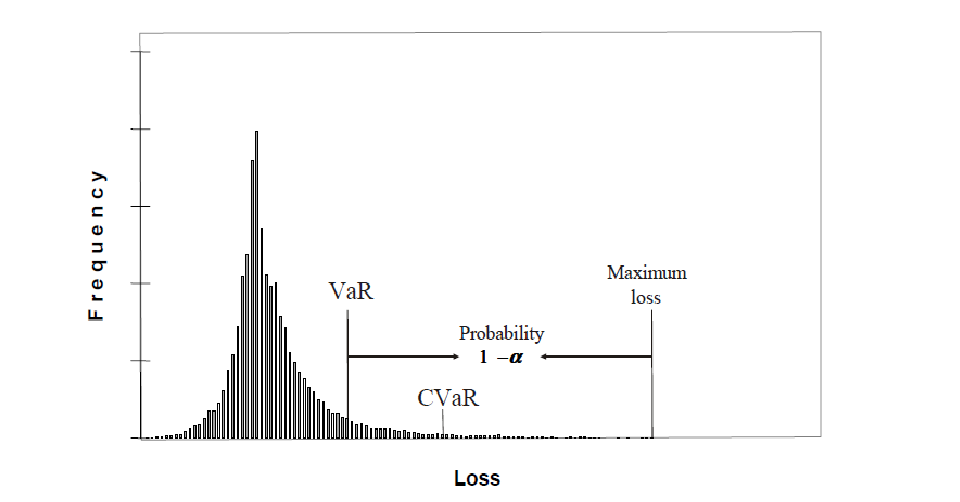
\includegraphics[width=0.95\linewidth]{figures/cvar.png}
	\caption{VaR and CVaR}\label{figvar}
\end{figure}

Note however that VaR is used in the finance sector where the underlying assets are usually liquid and the risky position can be closed at any time. This is not true when the underlying asset is a wind farm. The wind farm represents a physical asset that cannot be traded away quickly. This lack of liquidity for the underlying asset makes the use of the term \emph{value} misleading. Moreover, we are interested in analyzing the risk for the wind farm in terms of the possibility of low cash flows in the future. Therefore extend the concept of value at risk into the cash flow domain to obtain conditional cash-flow at risk (CCFaR) \cite{prokopczuk_quantifying_2007} as our risk measure. The expression for CCFaR (and cash-flow at risk, which is needed in defining CCFaR) with a given confidence level $\alpha$ is as follows. 
\begin{equation}
\begin{array}{ccl}
\text{CFaR}_\alpha &=& \text{sup}\{ \gamma : Prob(\text{Cash Flow} \leq \gamma) \leq 1 - \alpha\} \\
\text{CCFaR}_\alpha &=& E \left[\text{Cash Flow} | \text{Cash Flow} \leq \text{CFaR}_\alpha \right].
\end{array}
\end{equation}

Note that we have redefined the measures on the profit distribution rather than on the loss distribution. Therefore when considering the problem of maximizing profit while at the same time minimizing risk, we may use a weighted sum of the expected profit and the CCFaR as our utility. This follows from the fact that the higher the CCFaR the lower the probability of the profit falling below it.

Consider the utility function given by
\begin{equation*}
	\begin{array}{ccl}
		U(\pi) &=& \mu (\pi) + \kappa \ \text{CCFaR}(\pi),
	\end{array}
\end{equation*}

\noindent where $\mu(\pi)$ is the expected profit and CCFaR$(\pi)$ is the conditional cash flow at risk. We use a different risk aversion factor $\kappa$ than that in the mean-variance formulation ($\lambda$) to indicate that the two risk-aversion factors are not the same in general. The estimation of risk-aversion factors is beyond the scope of this paper, and will be addressed in future research.

The utility differential for the seller can then be given as 
\begin{equation} \label{util1}
\begin{array}{ccl}
\Delta U^S & = & U^S(\pi_C^S(p_C, q_C; \omega)) - U^S(\pi_{NC}^S(p_C, q_C; \omega)) \\
& = & E\displaystyle \sum_{t=1}^T \delta_t \left[p_C - p_t(\omega) \right]q_C + \kappa^S \left[\text{CCFaR}(\pi_C^S(p_C, q_C; \omega)) - \text{CCFaR}(\pi_{NC}^S(p_C, q_C; \omega))\right].
\end{array}
\end{equation}
\noindent Similarly the utility differential for the buyer can be given as 
\begin{equation} \label{util2}
\begin{array}{ccl}
\Delta U^B & = & U^B(\pi_C^B(p_C, q_C; \omega)) - U^B(\pi_{NC}^B(p_C, q_C; \omega)) \\
& = & \E \displaystyle \sum_{t=1}^T \delta_t \left[p_t(\omega) - p_C\right]q_C + \kappa^B \left[\text{CCFaR}(\pi_C^B(p_C, q_C; \omega)) - \text{CCFaR}(\pi_{NC}^B(p_C, q_C; \omega))\right].
\end{array}
\end{equation}

With the utility functions for the two parties defined as above, we are now ready to give the modeling framework for the negotiation process that determines the equilibrium structure of the CFD contract.

\section{Nash Bargaining Formulation}

Bargaining situations involve agents who engage in negotiations seeking mutual
benefit. Typically in such situations, no agent can take unilateral actions
without the consent of the other agents involved. This implicit coordination for
mutual benefit lends itself to natural game theoretic formulations for
bargaining. Two party bargaining games can be modelled using two distinct
paradigms - the static axiomatic approach and the dynamic strategic approach.
The static approach has its origins in the work of \cite{nash_bargaining_1950},
which describes the equilibrium solution to the problem by postulating certain
axioms that such a solution must satisfy. In contrast,
\cite{rubinstein1982perfect} proposed a sequential game model where the process
of offers and counter offers is treated explicitly as a dynamic game. Perfect
equilibria to such games are then treated
as solutions to the bargaining problem. 

In this paper, we focus on applying Nash's bargaining approach to the problem of
determining possible outcomes for wind hedge contracts
as described in Section~\ref{S:contract-model}. Given an $F$ player bargaining
problem, the axiomatic approach given in \cite{nash_two-person_1953}
characterizes the solution using the information given in the agents'
von Neumann-Morgenstern utility functions $(\pi_1, \pi_2, \ldots, \pi_F)$, the
set of allowable utilities $\prod_{f=1}^F\Gamma_f$ and a tuple of utility levels
$(\nu_1, \nu_2, \ldots, \nu_F)$ which represent the disagreement or threat
point. Under certain assumptions Nash showed that the bargaining problem has a
unique solution satisfying the axioms if and only if the payoffs to the players
are as follows.
\vspace*{-6pt}
\begin{equation}\label{eq:NBOpt}
\pi^* := (\pi_1^*, \ldots, \pi_F^*)\in \amax_{\nu \leq \pi\in \Gamma} \prod_{f=1}^F(\pi_f - \nu_f), \vspace*{-6pt}
\end{equation}
where $\Gamma=\displaystyle \prod_{f=1}^F\Gamma_f$ 

For two-player bargaining situations, the Nash bargaining solution (NBS) was
shown to be unique under the assumption that the feasible utility set of each
party is a non-empty, compact, convex subset of $\mathbb{R}^2$
\citep{nash_bargaining_1950, nash_two-person_1953}. Nash bargaining theory is
extended to non-convex problems, and various relaxations to the axioms are
explored in \cite{herrero_nash_1989, zhou_nash_1997} and \cite{mariotti_extending_1998}.

The utility differential maximization problem in \eqref{eq:NBOpt} provides the
equilibrium solution to the Nash bargaining problem in the space of utility
tuples. However, as a practical matter, we are interested in solving the problem
in the domain of the decision variables $p_C$ and $q_C$. Given the utility functions
from Section~\ref{S:contract-model}, we can formulate the Nash Bargaining
problem as maximizing the product of the utility differentials for the two
parties over the feasible regions of $p_C$ and $q_C$ so long as the
utility differentials for both parties are non-negative.

For notational simplicity the utility differentials from equations \eqref{util1} and \eqref{util2} are re-organized as follows.
\begin{equation}
\Delta U^S = \underbrace{\displaystyle \left( \E \left[ \sum_{t=1}^T \delta_t
	\left[p_C - p_t(\omega) \right]q_C \right]  - \kappa^S
	\text{CCFaR}(\pi_{NC}^S)\right)}_{\Psi^S(p_C, q_C)} + \kappa^S
\text{CCFaR}(\pi_C^S(p_C, q_C; \omega)).\\
\end{equation}
\begin{equation}
\Delta U^B = \underbrace{\displaystyle \left( \E \left[ \sum_{t=1}^T \delta_t
	\left[p_t(\omega) - p_C\right]q_C \right]  - \kappa^B
	\text{CCFaR}(\pi_{NC}^B)\right)}_{\Psi^B(p_C, q_C)} + \kappa^B
\text{CCFaR}(\pi_C^B(p_C, q_C; \omega)).
\end{equation}
Here the $\Psi$ terms are given by:
\begin{equation}
\begin{array}{rcl}
\Psi^S(p_C, q_C) & = & \E \left[\displaystyle \sum_{t=1}^T \delta_t \left[p_C -
p_t(\omega) \right]q_C \right]  - \kappa^S \text{CCFaR}(\pi_{NC}^S),\
\mathrm{and} \\ [15pt] 
\Psi^B(p_C, q_C) & = & \E \left[ \displaystyle \sum_{t=1}^T \delta_t
\left[p_t(\omega) - p_C\right]q_C \right] - \kappa^B \text{CCFaR}(\pi_{NC}^B).
\end{array}
\end{equation}
\noindent Using this notation the Nash Bargaining Solution (NBS) problem can be formulated as 
\begin{equation}\label{NBSReform11}
\begin{array}{cl}
\maximize{p_C,\ q_C \geq 0} & \dps \prod_{i \in \{S,B\}} \left[\Psi^i(p_C, q_C) + \kappa^i \text{CCFaR}(\pi_{C}^i(p_C, q_C; \omega))\right] \\
\st &\ \Psi^i(p_C, q_C) + \kappa^i \text{CCFaR}(\pi_{C}^i(p_C, q_C; \omega))
\geq 0, \quad \text{for} \ i \in \{S,B\}.
\end{array}
\end{equation}

\noindent As given in \eqref{NBSReform11}, the NBS problem is a stochastic
programming problem with expected value terms in $\Psi^i$ as well as conditional
expectation terms in the two CCFaR terms. The latter present an interesting
challenge in the context of optimization, since the decision variables $(p_C,
q_C)$ and the random variables $\omega$ cannot be decomposed. However,
\cite{rockafellar_optimization_2000} showed that the CCFaR terms may be
expressed in terms of expected value functions by
using the following auxiliary functions.
\begin{equation*}
	\begin{array}{ccl}
		\Gamma^S (p_C, q_C, \tau^S) &= &\displaystyle \tau^S - \frac{1}{1 - \alpha} E[\tau^S - \pi_C^S(p_C, q_C; \omega)]^+;\\[10pt]
		\Gamma^B (p_C, q_C, \tau^B) &= &\displaystyle \tau^B - \frac{1}{1 - \alpha} E[\tau^S - \pi_C^B(p_C, q_C; \omega)]^+,
	\end{array}
\end{equation*}
\noindent where $[\cdot]^+$ is defined as maximum between the argument in $[\ ]$
and 0. 

It can be shown that the CCFaR terms in \eqref{NBSReform11} may be replaced with
the corresponding $\Gamma$ terms. The optimization is then done over the
decision variables $(p_C, q_C)$ as well as the auxiliary variables $(\tau^S,
\tau^B)$. In order to show that this procedure results in an equivalent
formulation for the NBS problem, we first give a characterization of CCFaR in terms of the
auxiliary function $\Gamma$, as first given in \cite{rockafellar_optimization_2000}.

\begin{lemma}\label{lemma11}\citep{rockafellar_optimization_2000} \\
	Under the assumption that the probability distribution for the underlying uncertainty factors is continous, $\Gamma^i(p_C, q_C, \tau^i)$ is a convex, continuously differentiable function in $\tau^i$. The $\alpha$-CCFaR of the profit associated with a feasible $(p_C, q_C)$ pair can be determined from the formula
	\begin{equation*}
		\text{CCFaR}_{\alpha}(\pi_C^S(p_C, q_C; \omega)) = \maximi{\tau^i} \Gamma^i (p_C, q_C, \tau^i).
	\end{equation*}
	In this formula, the set consisting of the values of $\tau^i$ for which the maximum is attained, namely
	\begin{equation*}
		A_{\alpha}(p_C, q_C) := \displaystyle \amax_{\tau^i} \Gamma^i(p_C, q_C, \tau^i),
	\end{equation*}
	is a non-empty, closed and bounded interval (perhaps reduced to a single point), and the $\alpha$-CFaR of the profit is given by
	\begin{equation*}
		CFaR_{\alpha}(\pi^S_C(p_C, q_C; \omega)) = \displaystyle \supe_{\tau^i} (A_{\alpha}(p_C, q_C)).
	\end{equation*}
\end{lemma} 

\noindent Using Lemma \ref{lemma11}, we now proceed to show that the Nash
bargaining problem~\eqref{NBSReform11} can be reformulated in terms of the
auxiliary functions $\Gamma^i$ and the corresponding additional variables
$\tau^i$. 
\begin{proposition}\label{prop1}
	Solving the NBS problem~\eqref{NBSReform11} is equivalent to solving the
	following problem -
	\begin{equation}\label{eq:NBSReform1}
	\begin{array}{cl}
	\maximize{p_C,\ q_C, \ \tau^S,\ \tau^B} & \prod_{i \in \{S,B\}} \left[\Psi^i(p_C, q_C) + \kappa^i \Gamma^i (p_C, q_C, \tau^i)\right] \\
	\st & \Psi^i(p_C, q_C) + \kappa^i \Gamma^i (p_C, q_C, \tau^i) \geq 0 \quad \text{for} \ i \in \{S,B\} \\
	& p_C \geq 0, \ q_C \geq 0.
	\end{array}
	\end{equation}
\end{proposition}
\proof{Proof.}
\noindent Using Lemma \ref{lemma11}, we can replace the CCFaR terms in \eqref{NBSReform11} with the auxiliary function as follows
\begin{equation}\label{reform1}
\begin{array}{cl}
\maximize{p_C, \ q_C} & \prod_{i \in \{S,B\}} \left[\Psi^i(p_C, q_C) + \kappa^S \maximi{\tau^i} \Gamma^i (p_C, q_C, \tau^i)\right] \\
\st & \Psi^i(p_C, q_C) + \kappa^i \maximi{\tau^i} \Gamma^i (p_C, q_C, \tau^i) \geq 0 \quad \text{for} \ i \in \{S,B\}. \\
& p_C \geq 0, \ q_C \geq 0.
\end{array}
\end{equation}
We show that \eqref{reform1} is equivalent to \eqref{eq:NBSReform1} by making
the following observations. Firstly, $\Psi^i(p_C, q_C)$ is independent of
$\tau^i $ for $i \in \{S, B\}$. Therefore, we can take the inner `max' term out
of the objective function Secondly, we can relax the `max' term within the
constraints. Indeed it is easy to see that the constraint set for
\eqref{eq:NBSReform1} is a relaxation of the constraint set for \eqref{reform1},
since the only allowable $\tau^i$ in the
latter are maximizers for the corresponding $\Gamma^i$ terms. It suffices then
to show that any optimal solution to \eqref{eq:NBSReform1} is feasible to
\eqref{reform1}.

Suppose now that $(p_C^*, q_C^*, \tau^*)$ is optimal to problem
\eqref{eq:NBSReform1}. Let there be a $\tau$ such that $\Gamma^i(p_C^*, q_C^*,
\tau^i) > \Gamma^i(p_C^*, q_C^*, {\tau^*}^i)$ for $i = S$ or $i = B$ (or both).
Clearly $(p_C^*, q_C^*, \tau)$ is feasible to problem \eqref{eq:NBSReform1}
since 
\begin{equation} \label{tauopt}
\Psi^i(p_C^*, q_C^*) + \kappa^i \Gamma^i (p_C^*, q_C^*, \tau^i) > \Psi^i(p_C^*,
q_C^*) +
\kappa^i \Gamma^i (p_C^*, q_C^*, {\tau^*}^i) \geq 0.
\end{equation}
Moreover, \eqref{tauopt} also implies that
\begin{equation*}
	\prod_{i \in \{S,B\}} \left[\Psi^i(p_C^*, q_C^*) + \kappa^i \Gamma^i (p_C^*,
	q_C^*,
	\tau^i)\right] > \prod_{i \in \{S,B\}} \left[\Psi^i(p_C^*, q_C^*) + \kappa^i
	\Gamma^i (p_C^*, q_C^*, {\tau^*}^i)\right].
\end{equation*}
Since this contradicts the optimality of $(p_C^*, q_C^*, \tau^*)$ to
\eqref{eq:NBSReform1}, it is easy to see that ${\tau^*}^i \in \amax_{\tau_i}
\Gamma^i(p_C^*, q_C^*, \tau^i)$. 

We have thus shown that any optimal solution to the relaxation
\eqref{eq:NBSReform1} is feasible to \eqref{reform1}. Hence, the two problems
\eqref{NBSReform11} and \eqref{eq:NBSReform1} are equivalent.
\endproof

By Proposition \ref{prop1}, the solutions to problem~\eqref{eq:NBSReform1}
provide the equilibrium contract price $p_C$ and quantity $q_C$.
In order to simply analysis of the NBS problem, we restrict the feasible set to
be compact using the following argument. We make the assumption that the random
values taken on by the spot price $p_t(\omega)$ and the wind power output
$K_t(\omega)$ are bounded. Under this assumption, it is easy to see that the
variables $\tau^i$ are also bounded since at optimality these variables
represent the cash-flow at risk for each party. Moreover, it is then possible to
propagate the bounds on $p_C, q_C, \tau^S$ and $\tau^B$ to the variables $v^S$
and $v^B$. We add these implicit bounds on the variables, and use dummy
variables $v^S$ and $v^B$ to restrict the random functions to the constraints to
obtain the following reformulation to the NBS problem \eqref{eq:NBSReform1}.
\begin{equation} \label{NBSReform_2}
\begin{array}{cl}
\maximize{p_C,\ q_C,\ v^B,\ v^S,\ \tau^B,\ \tau^S} &  v^S v^B  \\
\st & \displaystyle v^i  \leq  \Psi^i(p_C, q_C) + \kappa^i  \Gamma^i (p_C, q_C,
\tau^i) \quad \text{for} \ i \in \{S,B\},\\%[20pt]
& 0 \leq p_C \leq \bar{p}_C, \\
& 0 \leq q_C \leq \bar{q}_C, \\
& \ubar{\tau}^i \leq \tau^i \leq \bar{\tau}^i, \quad i \in \{S,B\}, \\
& 0 \leq v^i \leq \bar{v}^i, \quad i \in \{S,B\}.
\end{array}
\end{equation}

Recall however that both the terms $\Psi^i(p_C, q_C)$ and $\Gamma^i(p_C, q_C)$
contain expected value terms taken with respect to the random vector $\omega$. Therefore,
problem \eqref{NBSReform_2} is a stochastic programming problem with expected
value constraints. For general probability distributions, analytical expressions
for these expectations are rarely available. In the following section, we
introduce sampling based techniques that can be utilized to solve this
problem.

\section{Sample Average Approximation}

The reformulated NBS problem~\eqref{NBSReform_2} falls under the classification
of expected value constrained stochastic programming problems. In their most
general form, such problems can be given as follows.
\begin{equation} \label{SP_expvalueconstr}
\begin{array}{ll}
\minimize{x \in X} & f(x) \\
\st & \E [g^i(x,\omega)] \leq 0 \quad \text{for } i = 1, \ldots, m.
\end{array}
\end{equation}
Here the non-empty set $X$ represents the deterministic constraints in the
decision variables $x$. It is implicitly assumed that the expected value
function $\E [g^i(x,\omega)]$ is well defined at all $x \in X$. 

To cast the reformulated NBS problem~\eqref{NBSReform_2} in this standard form,
let $x = (p_C, q_C, \tau^S, \tau^B, v^S, v^B)$, and let $X$ represent the bounds
on $x$. The objective function is then $$f(x) = f(p_C, q_C, \tau^S, \tau^B, v^S,
v^B) = v^S v^B$$. The constraint functions are given as follows.
\begin{equation} \label{constr_funs}
\begin{array}{rcl}
g^1(x, \omega) & = & v^S - \left[\displaystyle \sum_{t=1}^T \delta_t \left[p_C -
p_t(\omega) \right]q_C \right]  + \kappa^S \text{CCFaR}(\pi_{NC}^S) \\
& & \quad \quad \quad \quad \quad - \kappa^S
\left( \tau^S - \dps \frac{1}{1 - \alpha} [\tau^S - \pi_C^S(p_C, q_C; \omega)]^+
\right), \\ [10pt]
g^2(x, \omega) & = & v^B - \left[ \displaystyle \sum_{t=1}^T \delta_t
\left[p_t(\omega) + p_C\right]q_C \right] - \kappa^B \text{CCFaR}(\pi_{NC}^B) \\
& & \quad \quad \quad \quad \quad 
- \kappa^B \left( \dps \tau^B - \frac{1}{1 - \alpha} [\tau^S - \pi_C^B(p_C, q_C;
\omega)]^+ \right). 
\end{array}
\end{equation}
With this notation in place, it is straightforward to see how problem
\eqref{NBSReform_2} is of the form \eqref{SP_expvalueconstr}. 

In many practical applications, evaluating the expectation functions $\E[g^i(x,
\omega)]$ is either impossible due to the lack of analytical tractability or
prohibitively expensive computationally. Indeed, in our case, it is difficult to
obtain analytical expressions for the probability density functions for the wind
power output and spot electricity price vectors. However, historical data for
these parameters are readily available, and simulation models to generate
samples from such historical data have been well studied. The principle of
\emph{Sample Average Approximation} (SAA) utilizes such sampling schemes
combined with deterministic optimization methods to tackle stochastic
programming problems.

The fundamental idea behind SAA is to generate a random sample $\{\omega_1,
\omega_2, \ldots, \omega_N \}$ of $\omega$ and replace the expectations terms
$\E [g^i(x,\omega)]$ with the corresponding sample means. In other words,
instead of solving \eqref{SP_expvalueconstr}, we solve the following
deterministic problem -
\begin{equation} \label{SAA_general}
\begin{array}{ll}
\minimize{x \in X} & f(x) \\
\st & \dps  \frac{1}{N} \sum_{n=1}^N g^i(x,\omega_n) \leq 0 \quad \text{for } i
= 1, \ldots, m.
\end{array}
\end{equation}
Solutions to \eqref{SAA_general} serve as approximate solutions to
\eqref{SP_expvalueconstr} under appropriate assumptions. 

The origins of SAA as a technique for approximating stochastic programming
problems can be traced back to variants such as the stochastic counterpart
method \citep{rubinstein1993discrete} and sample path optimization
\citep{robinson1996analysis,plambeck1996sample,healy1991retrospective}. Under
mild assumptions, optimal solutions and the optimal value of the SAA problem can
be shown to converge to their true counterparts exponentially fast, for a
variety of stochastic programming problem classes. Using this theoretical
convergence rate, it is possible to estimate sample sizes required to
approximate solutions to the true problem with desired quality. The SAA problem
also provides avenues for statistically estimating bounds on the true optimal
objective value. It is therefore possible to provide solution quality guarantees
for the approximate solutions obtained by solving the SAA problem. For a summary
of the SAA approach and a comparison to alternative sampling approaches to
stochastic programming, we refer the reader to
\cite{shapiro_lectures_2009,Kim11aguide} and references therein.

The SAA approach has been used successfully in a variety of stochastic
programming settings including chance constrained problems
\citep{pagnoncelli2009sample}, problems with stochastic dominance constraints
\citep{hu2012sample}, and equilibrium/complementarity problems
\citep{gurkan1999sample,shapiro2008stochastic}. Convergence results for the SAA
approach were extended to the non-convex setting in
\cite{bastin_convergence_2006}.  In this paper, we focus mainly on solution
quality analysis for the SAA approach to expected value constrained
problems as laid out in \cite{wang_sample_2008}.

We seek to answer the following key questions regarding applying SAA to the NBS
problem~\eqref{NBSReform_2}.
\begin{enumerate}[label=(\roman*)]
	\item{As a practical matter, once an appropriate sample is generated, how does
		one solve the resulting SAA problem?}
	\item{What theoretical guarantees can one construct about the \emph{consistency}
		of optimal solutions and optimal values of the SAA problem to their true
		counterparts, as a function of growing sample size?}
	\item{Given finite termination of sampling at size $N$, what guarantees can be
		provided on the quality of the SAA solution generated?}
\end{enumerate}
We provide answers to these questions below.

\subsection{Solving the SAA Problem}

In this section, we discuss the deterministic optimization problem that results
from replacing the expected value terms in the NBS problem~\eqref{NBSReform_2}
with the corresponding sample averages. Suppose we generate $N$ samples of the
spot price and wind output capacity - $p^1, p^2, \ldots, p^N$ and $K^1, K^2,
\ldots, K^N$. Then the expectation terms in the $\Psi$ functions can be replaced
by a quadratic polynomial as follows.
\begin{equation}
\Psi_N^S(p_C, q_C) =  \displaystyle \left( \sum_{t=1}^T \delta_t  \right) p_C
q_C - \left( \frac{1}{N} \sum_{n=1}^N \sum_{t=1}^T p_t^n \right) q^C - \kappa^S
\text{CCFaR}_N(\pi_{NC}^S).
\end{equation}
Note that the term $\text{CCFaR}_N(\pi_{NC}^S)$ is simply a conditional
expectation taken on a discrete distribution of the payoffs without the
contract. Since these payoff terms do not contain the decision variables $p_C$
and $q_C$, $\text{CCFaR}_N(\pi_{NC}^S)$ resolves into a constant after the sampling.

In a similar fashion we resolve the $\Psi$ terms for the buyer as follows.
\begin{equation}
\Psi_N^B(p_C, q_C) = \displaystyle \left( \frac{1}{N} \sum_{n=1}^N \sum_{t=1}^T
p_t^n \right) q^C - \left( \sum_{t=1}^T \delta_t  \right) p_C q_C  - \kappa^B
\text{CCFaR}_N(\pi_{NC}^B).
\end{equation}

Now consider the auxiliary function terms $\Gamma^i(p_C, q_C, \tau^i)$.
\begin{equation}
\Gamma^i_N(p_C, q_C, \tau^i) = \tau^i - \frac{1}{1 - \alpha} E[\tau^i -
\pi_C^i(p_C, q_C)]^+ = \tau^i - \frac{1}{N(1 - \alpha)}\sum_{n=1}^{N} [\tau^i - \pi_C^i(p^n, K^n)]^+.
\end{equation}
Note that $\Gamma^i_N$ is non-differentiable because of the positive-part terms.
However we may use the standard trick of using auxiliary variables $z^i_n$ for
each positive-part term inside the summation, and construct a reformulation by
adding linear constraints in the $z$ variables. The resulting deterministic
equivalent to the NBS problem~\eqref{NBSReform_2} is given below.
\begin{equation} \label{NBSfinal}
\begin{array}{cl}
\maximize{p_C,\ q_C,\ v^B,\ v^S,\ \tau^B,\ \tau^S} &  v^S v^B  \\
\st & \displaystyle v^S  \leq  \Psi_N^S(p_C, q_C) + \kappa^S \left[ \tau^S - \frac{1}{N(1 - \alpha)} \displaystyle \sum_{n=1}^{N} z_n^S \right] \\[20pt]
& \displaystyle v^B  \leq  \Psi_N^B(p_C, q_C) + \kappa^B \left[ \tau^B - \frac{1}{N(1 - \alpha)} \displaystyle \sum_{n=1}^{N} z_n^B \right] \\[20pt]
& z_n^S  \geq  \tau^S - \pi_C^S(p^n, K^n) \quad \text{for} \quad n = 1 , \dots,  N \\
& z_n^B  \geq  \tau^B - \pi_C^B(p^n, K^n) \quad \text{for} \quad n = 1 , \dots,  N \\ [10pt]
& z_n^B, z_n^S  \geq  0 \quad \text{for} \quad n = 1 , \dots, N, \\
& 0 \leq p_C \leq \bar{p}_C, \\
& 0 \leq q_C \leq \bar{q}_C, \\
& \ubar{\tau}^i \leq \tau^i \leq \bar{\tau}^i, \quad i \in \{S,B\}, \\
& 0 \leq v^i \leq \bar{v}^i, \quad i \in \{S,B\}.
\end{array}
\end{equation}
We observe here that it is easy to find an initial feasible solution for the
problem \eqref{NBSfinal}.
\begin{lemma}
	Setting $p_C$ and $q_C$ to 0 will always result in a feasible solution for \eqref{NBSfinal}.
\end{lemma}
\proof{Proof.}
Given $p_C = q_C = 0$, set $\tau^i$ to the corresponding Cash-Flow-at-Risk level
$\text{CFAR}^i_{\alpha}$. Now let 
\begin{equation*}
	z_n^i = [\tau^i - \pi_C^i(p_n, q_n)]^+.
\end{equation*}
Then using Lemma \ref{lemma11} and Proposition \ref{prop1}, we have that
\begin{equation*}
	\left[ \tau^i - \frac{1}{N(1 - \alpha)} \displaystyle \sum_{n=1}^N z_n^i \right]
	= \text{CCFaR}_\alpha (\pi_C^i(p_C, q_C)) \ \ \text{for } \ i \in \{S,B\}
\end{equation*}
under the given sampling. Note also that setting $q_C = 0$ implies that payoffs
with and without the contract are the same.
\begin{equation*}
	\pi_C^i(p_C, q_C) = \pi_{NC}^i(p_C, q_C).
\end{equation*}
Now consider the utility differential variables $v^i$. Let
\begin{equation*}
	\begin{array}{ccl}
		v^i & = & \displaystyle \Psi^i(p_C, q_C) + \kappa^i \left[ \tau^i - \frac{1}{N(1
			- \alpha)} \displaystyle \sum_{n=1}^N z_n^i \right] \ \ \text{for } \ i \in \{S,B\} \\
		& = & \Psi^i(p_C, q_C) + \kappa^i \text{CCFaR}_\alpha (\pi_{NC}^i).
	\end{array}
\end{equation*}
Note that 
\begin{equation*}
	\begin{array}{ccl}
		\Psi^i(p_C, q_C)  & = & \E \displaystyle \sum_{t=1}^T \delta_t \left[p_C - p_t(\omega) \right]q_C - \kappa^S \text{CCFaR}_\alpha(\pi_{NC}^i) \\
		& = & - \kappa^S \text{CCFaR}_\alpha(\pi_{NC}^i),
	\end{array}
\end{equation*}
since $q_C = 0$.
Thus it is easily seen that $v^i = 0$. So the above assignments of $z^i_n$,
$\tau_i$ and $v^i$ for $i \in \{S,B\}$ always provide a feasible solution to
problem \eqref{NBSfinal}. 
\endproof

The NBS SAA problem~\eqref{NBSfinal} is non-convex due to the bilinear terms in
$\Psi^i_N(p_C,q_C)$. In general obtaining globally optimal solutions to such
problems is difficult. However, there exist several techniques such as
reformulation-linearization methods \citep{sherali1992new}, cutting plane
algorithms \citep{konno1976cutting}, and outer-approximations
\citep{Floudas1995} that can handle bilinear optimization
problems. Since several such methods are incorporated into standard global
optimization solvers such as BARON or COUENNE, we henceforth make the
assumption that the SAA problem is solved to global optimality for any given
sample.

\subsection{Consistency of SAA estimators} \label{S:SAAcons}

In this section, we analyze the behaviour of optimal solutions and the optimal
value to the SAA problem~\eqref{NBSfinal} as the sample size $N$ is increased
(in theory to $\infty$). Denote by $\nu^*$ and $S^*$ the optimal value and the
set of optimal solutions to the true problem \eqref{NBSReform_2}. Let
$\nu_N$ and $S_N$ be the optimal value and the set of optimal solutions to the
SAA problem \eqref{NBSfinal}. The main question we wish to answer is whether
$v_N$ and $S_N$ converge, in an appropriate sense, to their true counterparts as
$N \to \infty$. 

We establish the desired consistency for our SAA problem by
relying on the following general result for stochastic
programming problems, as given in \cite{shapiro_lectures_2009}. Consider the
generic problem~\eqref{SP_expvalueconstr} and the corresponding deterministic
equivalent~\eqref{SAA_general}. Let $X_N = \{ x \in X \ | \
N^{-1} \sum_{n=1}^N g^i(x, \omega_n) \leq 0, \ i=1,\ldots,m \}$ and $\bar{X} =
\{ x \in X \ | \ \E [ g^i(x, \omega)] \leq 0, \ i=1,\ldots,m \}$

\begin{theorem} \label{SAAcons} \citep{shapiro_lectures_2009}
	Suppose that there exists a compact set $C \in \Real^d$ such that: 
	\begin{enumerate}[label=(\roman*)]
		\item{The set $S^*$ of optimal solutions of the true problem is nonempty and
			contained in $C$,}
		\item{The function $f(x)$ is continuous and finite valued on $C$, and}
		\item{With probability 1 for $N$ large enough the set $S_N$ is nonempty
			and contained in $C$.} 
	\end{enumerate}
	Suppose further that constraint sets $X_N$ satisfy the following conditions
	- 
	\begin{enumerate}[label=(\roman*)]
		\setcounter{enumi}{3}
		\item{If $x_n \in X_N$ and $x_N \to x$ with probability 1, then $x \in \bar{X}$, and}
		\item{For some $x \in S^*$ there exists a sequence $x_N \in X_N$ such that $x_N
			\to x$ with probability 1.} 
	\end{enumerate}
	Then $\nu_N \to \nu^*$ and $\D(S_N, S^*) \to 0$ with probability 1 as $N \to
	\infty$. 
\end{theorem}
Note that $\D(A,B)$ denotes the deviation of set $A$ from set $B$.

In applying Theorem \ref{SAAcons} to problem \eqref{NBSReform_2} the set $X$ is an obvious choice for $C$. Any feasible solution to both the true
problem \eqref{NBSReform_2} and the SAA problem \eqref{SAA_general} must lie in
$X$. Thus we have $S^* \subset X$ and $S_N \subset X$. 
The objective function $f$ is a bilinear function and must therefore be continuous
on $X$. Moreover, since $v^S$ and $v^B$ are bounded, $f$ must also be bounded on
$X$. This takes care of condition $(ii)$.

If for a given point $x \in X$, the functions
$\bar{g}_N^i(x) = N^{-1} \sum_{n=1}^N g^i(x, \omega_n)$ converge uniformly to
the true constraint functions $\bar{g}^i(x) = \E[g^i(x,\omega)]$ with
probability 1 on a neighborhood of $x$, and the functions $\bar{g}^i$ are
continuous, then it can be shown that condition $(iv)$ of Theorem \ref{SAAcons} is satisfied. Both the
uniform convergence and continuity properties may be established using the
following result.

\begin{theorem} \label{expvalueunifconv} \citep{shapiro_lectures_2009}
	Let $X$ be a nonempty compact subset of $\Real^d$ and suppose that 
	\begin{enumerate}[label=(\roman*)]
		\item{for any $x \in X$, the functions $g^i(\cdot,\omega)$ are continuous at $x$ for
			almost every $\omega \in \Omega$,}
		\item{$g^i(x,\omega), x \in X$ are dominated by integrable functions
			$c^i(\omega)$, and}
		\item{the sample $\{ \omega_1, \ldots, \omega_N\}$ is i.i.d.}
	\end{enumerate}
	Then the expected value functions $\bar{g}^i(x)$ are finite valued and continuous
	on $X$, and $\bar{g}^i_N(x)$ converges to $\bar{g}^i(x)$ with probability 1
	uniformly on $X$.
\end{theorem}

Recall that the functions $g^i(x,\omega)$ as defined in \eqref{constr_funs} are
bilinear in $(p_C, q_C)$ and linear in $v^i$ and $\tau^i$ for each $\omega$.
Thus the continuity of $g^i(\cdot, \omega)$ for each $x$ and for every $\omega
\in \Omega$ is obvious. Moreover, it is easy to see that $| g^i(x, \omega) |
\leq 2 \bar{v}^i$ by construction of the bound $\bar{v}^i$. Thus we can set
$c^i(\omega) = \bar{v}^i$ to obtain the desired integrable functions to satisfy
condition $(ii)$ in Theorem \ref{expvalueunifconv}. Thus we have shown that if
the sampling is i.i.d then condition $(iv)$ of Theorem \ref{SAAcons} holds.

The continuity of $\bar{g}^i(x)$ also implies that the constraint set $\bar{X}$
is compact. Furthermore, it is easy to see that setting $q_C = 0$ will result in
both utility differentials being 0. Since this provides a feasible point $x_0$ in
$\bar{X}$, it is easy to see that $S^*$ must be non-empty. Thus condition $(i)$
is verified.

Noting that the functions $\bar{g}^i_N(x)$ are simply summations of polynomial
terms, it is easy to see that the set $X_N$ must also be compact. Moreover, the
point $x_0$ with $q_C = 0$ remains feasible irrespective of the sampling, i.e.
$x_0 \in X_N$. This means that the set $S_N$ must be non-empty. 

In order to verify the remaining condition $(v)$, we utilize an implicit
assumption that there exists a decision tuple $(p_C, q_C)$ which results in a
strictly positive utility differential for both parties. By this assumption,
there must certainly be an equilibrium solution $\bar{x} \in S^*$ with the same
positive utility differential property. Formally, let
$\bar{g}^i(\bar{x}) = - \epsilon^i < 0$ for $i \in \{S,B\}$. Then, by the strong law
of large numbers, we must have a finite $N_0$ such that 
\[ | g^i_N(\bar{x}) - \bar{g}^i(\bar{x}) | < \epsilon^i, \quad \forall N > N_0. \]
But this clearly implies that 
\[ g^i_N(\bar{x}) < \epsilon^i + \bar{g}^i(\bar{x}) = 0, \quad \forall N > N_0. \]
In other words, for all $N > N_0$, $\bar{x} \in X_N$. Clearly, as long as we set
$x_N = \bar{x}$ for $N > N_0$, it easy to construct the desired sequence
$\{x_N\}$ to satisfy condition $(v)$.

\subsection{Convergence Rate and Solution Quality}

While the consistency of the optimal values $\nu_N$ and the solution sets $S_N$
to their true counterparts is certainly reassuring, practical
implementations of the SAA method must necessarily terminate with a finite
sample size $N$. In this case, it is important to ascertain the quality of the
solution generated with respect to both feasibility as well as optimality to the
true problem. 

In general, while applying the SAA principle to expected value constrained
problems, it is not possible to guarantee that the solution to the SAA problem
with a finite sample size $N$ is feasible to true problem. Thus the main
quantity of interest is the probability that the candidate solution in question
is $\epsilon-$feasible to the true problem. Furthermore, it is desired that the
approximation obtained from the SAA problem is not too conservative. The main
techniques to derive bounds on this probability is the theory of large
deviations. The results we present in this section are outlined
in detail in \cite{wang_sample_2008}.

Consider the SAA problem \eqref{SAA_general}. Let $\bar{X}^{\epsilon} := \{x \in
X \ | \ \bar{g}^i(x) \leq \epsilon, \text{ for } i = 1, \ldots, m \}$ and
$X_N^{\epsilon} := \{x \in X \ | \ g^i_N(x) \leq \epsilon, \text{ for } i = 1,
\ldots, m \}$. Then we wish to estimate the probability
$p = \text{Pr}(\bar{X}^{-\epsilon} \subseteq X_N^0 \subseteq \bar{X}^{\epsilon})$
for finite $N$, i.e. the probability that a feasible point to the
problem~\eqref{SAA_general} is $\epsilon$-feasible to the true stochastic
problem. 

Before stating the formal bounding results on $p$, we state the following
additional assumptions for solution quality analysis. 
\begin{enumerate}[label=(\roman*)]
	\setcounter{enumi}{5}
	\item{For any $x \in X$, the moment generating function of $g^i(x,\omega) -
		\bar{g}^i(x)$ is finite in a neighborhood of zero.}
	\item{For any $\omega \in \Omega$, there exists an integrable function $\phi:
		\Omega \to \Real_+$ such that 
		\[ | g^i(x_1, \omega) - g^i(x_2, \omega) | \leq \phi(\omega) \norm{x_1 - x_2}, \
		\forall x_1, x_2 \in X. \] Let $\Phi := \E[\phi(\omega)]$.}
	\item{The moment generating function of $\phi(\omega)$ is finite in a
		neighborhood of zero.}
\end{enumerate}
It was shown in Section~\ref{S:SAAcons} we showed that $| g^i(x,\omega) | \leq 2 \bar{v}^i$ for any $\omega \in \Omega$. This certainly means that $| \bar{g}^i(x) | \leq 2 \bar{v}^i$. Combining the
two bounds, it is easy to see that $| g^i(x,\omega) - \bar{g}^i(x) | \leq 4
\bar{v}^i$. Using this bound, it is straightforward to show that assumption (vi)
is satisfied.

Assumption (vii) requires that the functions $g^i(x,\omega)$ are Lipschitz
continuous with respect to $x \in X$ for each $\omega \in \Omega$. This property is
easy to establish given that for fixed values of $\omega$, $g^i(\cdot, \omega)$
are polynomials in $x$. Moreover, since $X$ is closed and bounded and the random
vectors $p_t(\omega)$ and $K_t(\omega)$ are also bounded, we can set
\[ \phi(\omega) = L = \max_{x \in X, \omega \in \Omega} \norm{\nabla_x g^i(x,
	\omega)}. \]
This choice gives us the desired $\phi(\omega)$ for satisfying assumptions (vii)
and (viii).

Under the assumptions for Theorem~\ref{expvalueunifconv} as well as the
additional assumptions (vi)-(viii), the probability $p$ may be bounded
as follows.
\begin{theorem} \cite{wang_sample_2008} \label{SAAquality}
	Suppose (i) - (viii) hold. Define $\sigma^2 := \max_{x \in X}
	\{ \text{Var}[\phi(\omega)], \text{Var}[g^i(x,\omega) - \bar{g}^i(x)] \}$ and
	$\mu := (4 \Phi/ \epsilon + 1)^{-1}$. Given $\epsilon > 0$, we have 
	\[ Pr(\bar{X}^{-\epsilon} \subseteq X_N^0 \subseteq \bar{X}^{\epsilon}) \geq 1 -
	2\left( 1 + \frac{D^k}{\mu^k} \right) e^{-\frac{N \epsilon^2}{8 \sigma^2}}. \]
	Moreover, for a given confidence level $\beta$, if 
	\[ N \geq \frac{8 \sigma^2}{\epsilon^2} \log \left[ \frac{2}{\beta} \left( 1 +
	\frac{D^k}{\mu^k} \right) \right], \]
	then $  Pr(\bar{X}^{-\epsilon} \subseteq X_N^0 \subseteq \bar{X}^{\epsilon})
	\geq 1 - \beta$.
\end{theorem}
Here, $D$ is the diameter of the set $X$ and $k$ is a parameter representing
bounds on the cardinality of subsets $X_{\mu}$ such that any point in $X$ is
within a distance of $\mu$ from $X_{\mu}$.

The sampling size estimate obtained using Theorem \ref{SAAquality}, while
theoretically appealing, is often conservative in practice. Much better sample
size estimates can be obtained by performing statistical validation on candidate
solutions to the SAA problem.

Given a candidate solution to the SAA problem \eqref{NBSReform_2}, upper bounds
are computed using Lagrange duality. Any feasible solution to the true problem
gives valid lower bounds. Typical practice is to use solutions to the SAA
problem as candidate feasible solutions. In this case, the expected value
constraints must be ``loosened'' by an appropriate amount, in order to increase
the probability that the solution generated is feasible to the true problem.
We refer the reader to \cite{wang_sample_2008} for details of the
validation scheme. The scheme itself as applied to the problem
\eqref{NBSReform_2} is given below in Algorithm~\ref{A:SAA}. The parameter
$\tilde{z}$ is chosen for a desired upper-bound confidence probability $\beta$,
while $\tilde{\epsilon}$ is used for relaxing the expected value constraints.
The confidence level for lower bounding is given by $\gamma$.

\subsection*{SAA Scheme}

\begin{framed}
	\begin{enumerate}[label={\bf Step \arabic*}.]
		\item{\textbf{Initialize}: \\
			Set $\bar{z} > 0, \bar{\epsilon} > 0, \gamma \in (0,1)$. \\
			Generate a sample $(\omega_1, \omega_2, \ldots, \omega_N)$ of size $N$.} 
		
		\item{\textbf{Compute candidate dual multiplier}: \\
			Solve the SAA problem \eqref{SAA_general} to obtain an optimal primal-dual pair
			$(\tilde{x}, \tilde{\pi})$.}
		
		\item{\textbf{Estimate lower bounds}: \\
			Generate an independent sample of size $N_u$ for lower bound estimation. \\
			Compute \[ \tilde{u} = \bar{g}^i_{N_u} (\tilde{x}) = \frac{1}{N_u}
			\sum_{n=1}^{N_u} g^i(\tilde{x}, \omega_n), \]
			\[ S_u^2 (\tilde{x}) = \frac{1}{N_u(N_u - 1)} \sum_{n=1}^{N_u} [g^i(\tilde{x}, \omega_n) -
			\tilde{u}]^2, \text{ and }\]
			\[ z_{\beta} = \frac{- g_{N_u}(\tilde{x})}{S_u(\tilde{x})}. \] 
			If $z_{\beta} < \tilde{z}$, relax the SAA problem \eqref{SAA_general} by
			$\bar{\epsilon}$ and resolve.}
		
		\item{\textbf{Estimate upper bounds}: \\
			Generate $M_l$ independent samples each of size $N_l$ for lower bound
			estimation. \\
			For each sample $j = 1, \ldots, M_l$ , solve the SAA Lagrange problem
			\[\tilde{l}^j = \min_{x \in X} \left\{ f(x) + N_l^{-1} \sum_{i=1}^m \left( \tilde{\pi}^i
			\sum_{n=1}^{N_l} g^i(x,\omega_n) \right)\right\}. \] 
			Compute lower bound estimator $\tilde{l}$ and its variance $S_l^2$ as follows.
			\[ \tilde{l} = \frac{1}{M_l} \sum_{j=1}^{M_l} \tilde{l}^j, \]
			\[ S_l^2 = \frac{1}{M_l(M_l - 1)} \sum_{j=1}^{M_l} (\tilde{l}^j - \tilde{l})^2.
			\]\\
			Compute a $(1 - \gamma)$ confidence interval for $\E [\tilde{l}]$ as $\dps
			\left[ \tilde{l} - z_{\gamma / 2} S_{l}, \tilde{l} + z_{\gamma / 2} S_{l}
			\right]$.}
	\end{enumerate}
\end{framed}
One important aspect of the SAA scheme that we haven not addressed is the
computation of optimal dual multipliers $\tilde{\pi}$. Since the actual
deterministic equivalent solved is problem~\eqref{NBSfinal} rather than directly
on the sampled version of \eqref{NBSReform_2}, care needs to be taken to ensure
that the appropriate dual multipliers for \eqref{NBSReform_2} are found. We
assume here that once \eqref{NBSfinal} is solved using a global optimization
solver, the optimal primal variables can be used to explicitly compute the
dual multipliers for the utility differential constraints in \eqref{NBSReform_2}.

\section{Numerical Results}

In this section we present numerical results for the SAA method applied to the
wind hedge contract NBS problem. Our primary goal is to study how the
equilibrium structure for wind hedges evolve as various input parameters such as
risk aversion or market features change. To simplify this process, we use
a carefully controlled simulation model to generate wind power and spot electricity
prices. It must be noted that this model are grossly simplified and are
used for the explicit purpose of comparative statics analysis. For more accurate
state-of-the-art forecasting methods for wind power and spot electricity prices,
we refer the reader to
\cite{lei2009review,foley2012current,contreras2003arima,weron2007modeling} and
references therein.  

To begin with, we use a simple geometric
Brownian motion (GBM) model to generate wind power output and spot electricity prices.
The data generated from this model is then used to solve the SAA problem. By
carefully modifying the input to the GBM model, we are able to conduct
comparative statics studies on how parameters such as volatilities affect the
equilibrium outcomes to the problem. The spot price and wind output paths are generated using the input
data to the GBM model as given in Table~\ref{input_data}.
\begin{table}[htp!] \label{input_data}
	\caption{Parameters for forecasting data.}
	\begin{framed}
		\begin{tabular}{ll}
			$p^S$ & 50\$/MWhr - starting price for spot electricity. \\
			$K^S$ & 30 MW - starting point for wind output. \\
			$p_{dr}$ & 0.05 - drift in spot price. \\
			$K_{dr}$ & 0 - drift in wind output. \\
			$p_{\sigma}$ & 5\% - standard deviation in spot electricity price.\\
			$K_{\sigma}$ & 5\% - standard deviation in wind output.\\
			$corr(p, K)$ & -0.5 - correlation between electricity price and wind output.\\
			$\kappa^S$ & 5 - risk aversion for wind farm.\\
			$\kappa^B$ & 1 - risk aversion for buyer.
		\end{tabular}
	\end{framed}
\end{table}

The GBM model is used to construct sample paths for the wind power output and
spot electricity price. The data was generated using the MATLAB
financial toolbox on a Windows 7 machine with a quad core intel i7 processor and
8 GB of memory. The SAA problems were solved using the global optimization
solver BARON \citep{baron1} on the cloud optimization server NEOS
\citep{neos1,neos2,neos3}. 

We choose $\tilde{z} = 2.33$ corresponding to a
$99\%$ confidence required for the upper bound candidate solution to be
feasible. The parameter $\tilde{\epsilon}$ is chosen to be $1\%$ of the average
expected value constraints. For the lower bounding scheme, we choose a $95\%$
confidence interval. The sampling sizes are chosen as follows - $N = 300$, $N_u
= 3000$ and $N_l = 150$. For lower bounding, 10 different samples of size $N_l$
are generated. 

With the input data as indicated above, we obtain the following numerical
results. The upper bounding scheme took a total of $()$ iterations, where the
right hand side was modified to relax the expected value constraints. The
candidate solution obtained was $p_C = $ and $q_C = $, with a corresponding
upper bound of $UB = $. The left end point of the
$\gamma$-confidence interval for the lower bound is given by $LB = $. 

\subsection*{Comparative Statics}

\begin{figure}[htb]
	\begin{center}
		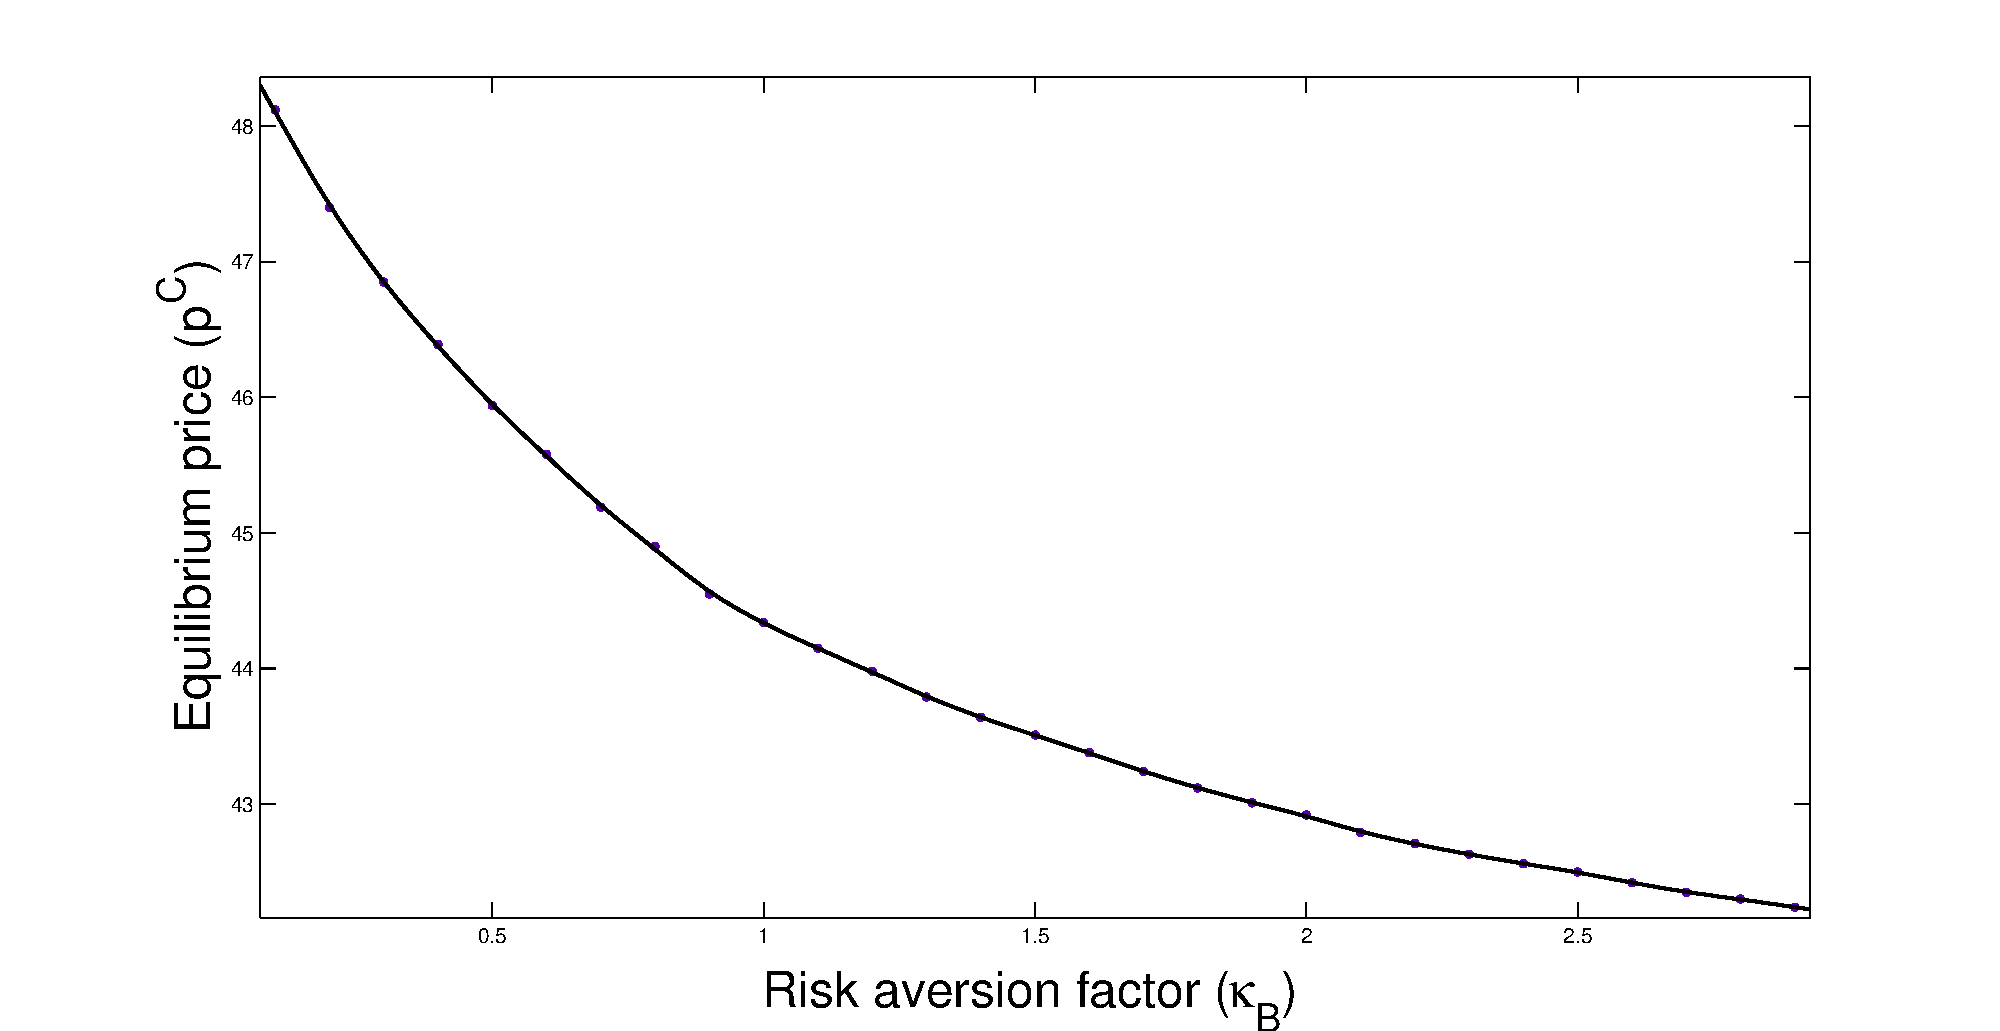
\includegraphics[height=3in]{figures/p_kb.pdf}
		\caption{$p_C$ vs $\kappa^B$} \label{pckb}
	\end{center}
\end{figure}
\begin{figure}[htb]
	\begin{center}
		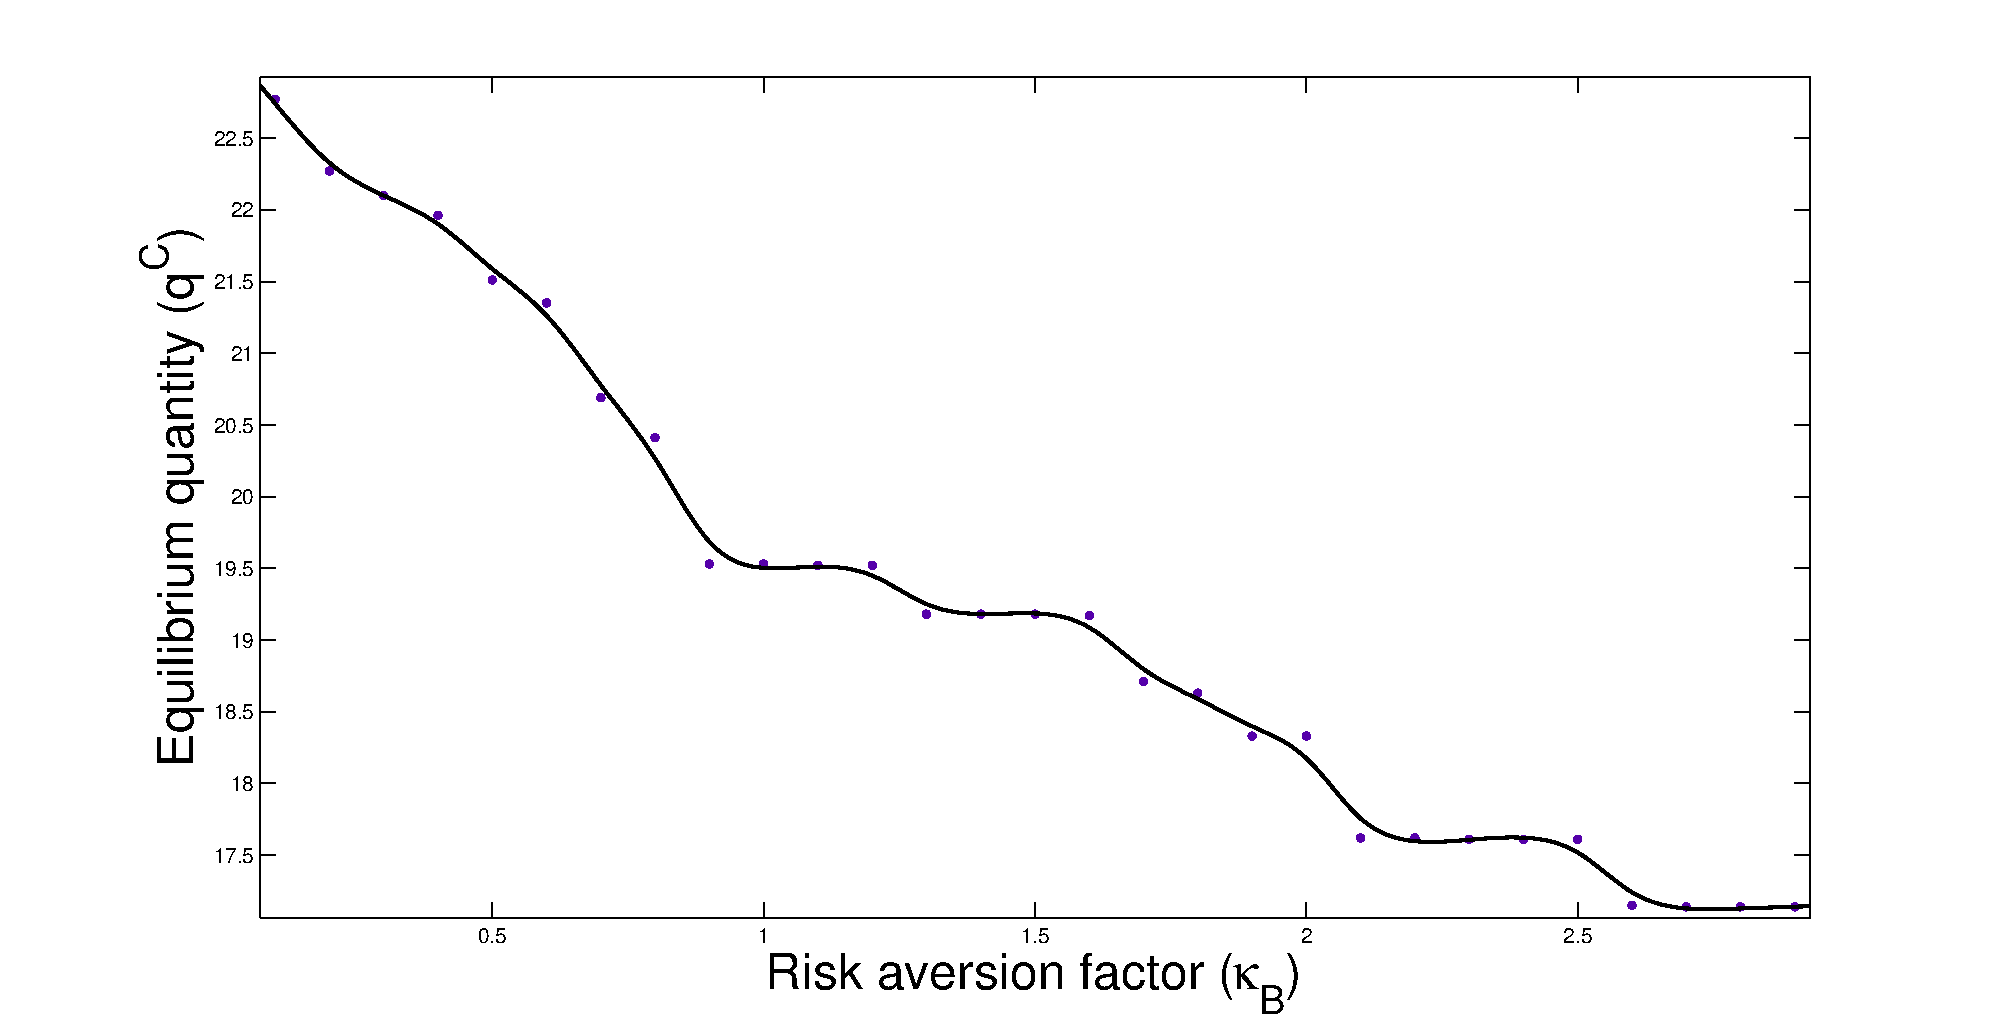
\includegraphics[height=3in]{figures/q_kb.pdf}
		\caption{$q_C$ vs $\kappa^B$} \label{qckb}
	\end{center}
\end{figure}

We also study the behavior of the NBS equilibrium solutions as some of the model
parameters are varied. Comparative statics analysis was done on the following
parameters - spot price and wind power output volatilities, risk attitudes of
the two parties and the correlation between wind power output and spot price. 

Figures \ref{pckb} and \ref{qckb} plot the equilibrium price and quantity
respectively, as the risk aversion parameter $\kappa^B$ for the buyer is varied.
As the buyer becomes less risk averse, it is willing to take on larger
quantities through the hedge at larger prices.  This results in larger profits
and less risk for the wind farm. From the buyer's perspective, as its risk
aversion increases, it demands a higher premium for the transfer of risk. The
higher premium appears in the form of a lower equilibrium price that the buyer
is willing to pay. Because the wind farm's risk aversion remains constant
throughout the experiment, a reduction in the price results in a reduction in
the quantity that the wind farm is willing to sell.

An increase in the wind farm's risk aversion produces a similar result on the
strike price. The wind farm is willing to pay a higher premium for the contract
in exchange for hedging more of its risk. However, the quantity does not
decrease since the wind farm is now willing to trade the same or higher
quantities even at the higher premium levels.

Market variations such as the volatility of the spot price affect both parties
equally. In this case, we expect to see opposing patterns in the equilibrium
price and quantity since a lowering of price and an increase of the quantity
both represent increased willingness to participate in the contract.
The variations in equilibrium structure as the spot price volatility is changed
is given in Figures \ref{pcpvol} and \ref{qcpvol}. As the spot price becomes
more volatile, the risk taken on by the wind farm increases. As a result of this
added risk, the wind farm becomes willing to pay higher premiums for the hedge
as well as to trade more of the risk away by increasing the quantity hedged.
This is illustrated by the downward sloping price curve and the upward sloping
quantity curve.

\begin{figure}[t]
	\begin{center}
		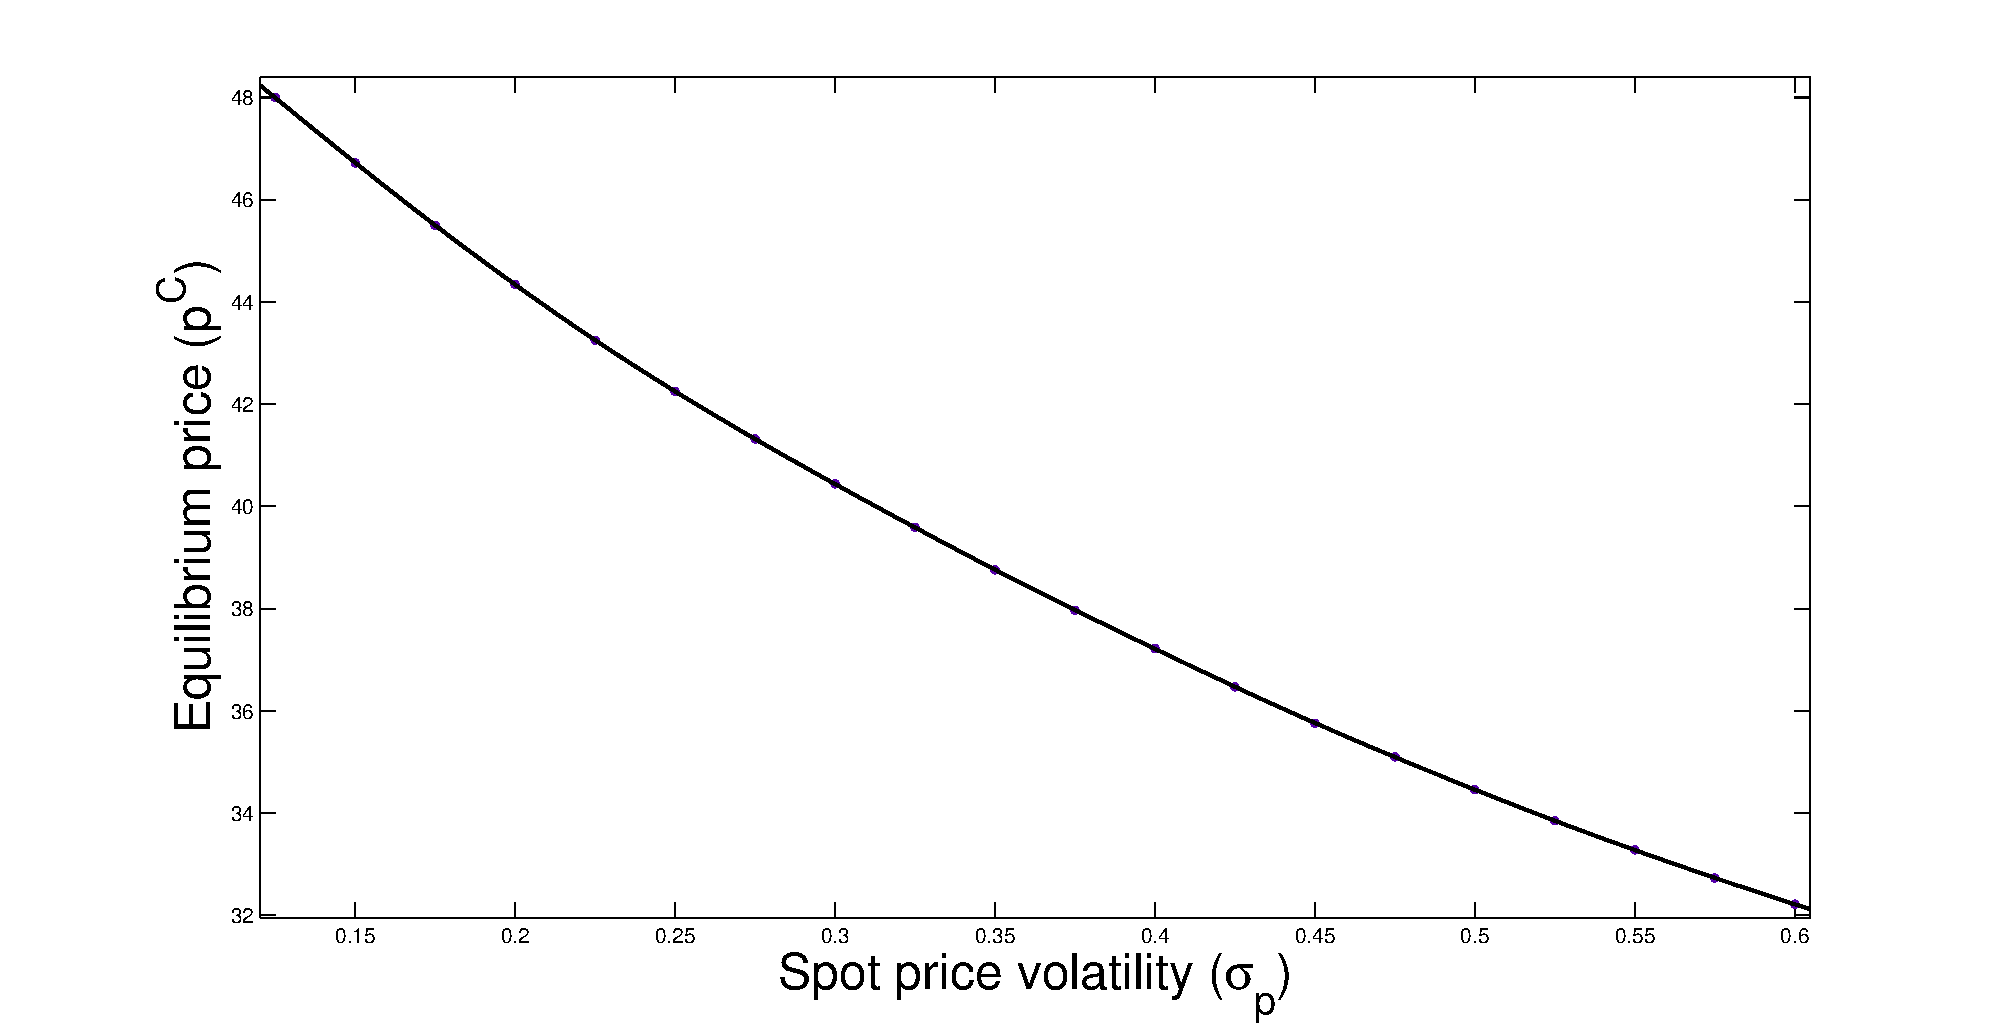
\includegraphics[height=3in]{figures/price_vol.pdf}
		\caption{$p_C$ vs $p_\sigma$} \label{pcpvol}
	\end{center}
\end{figure}
\begin{figure}[t]
	\begin{center}
		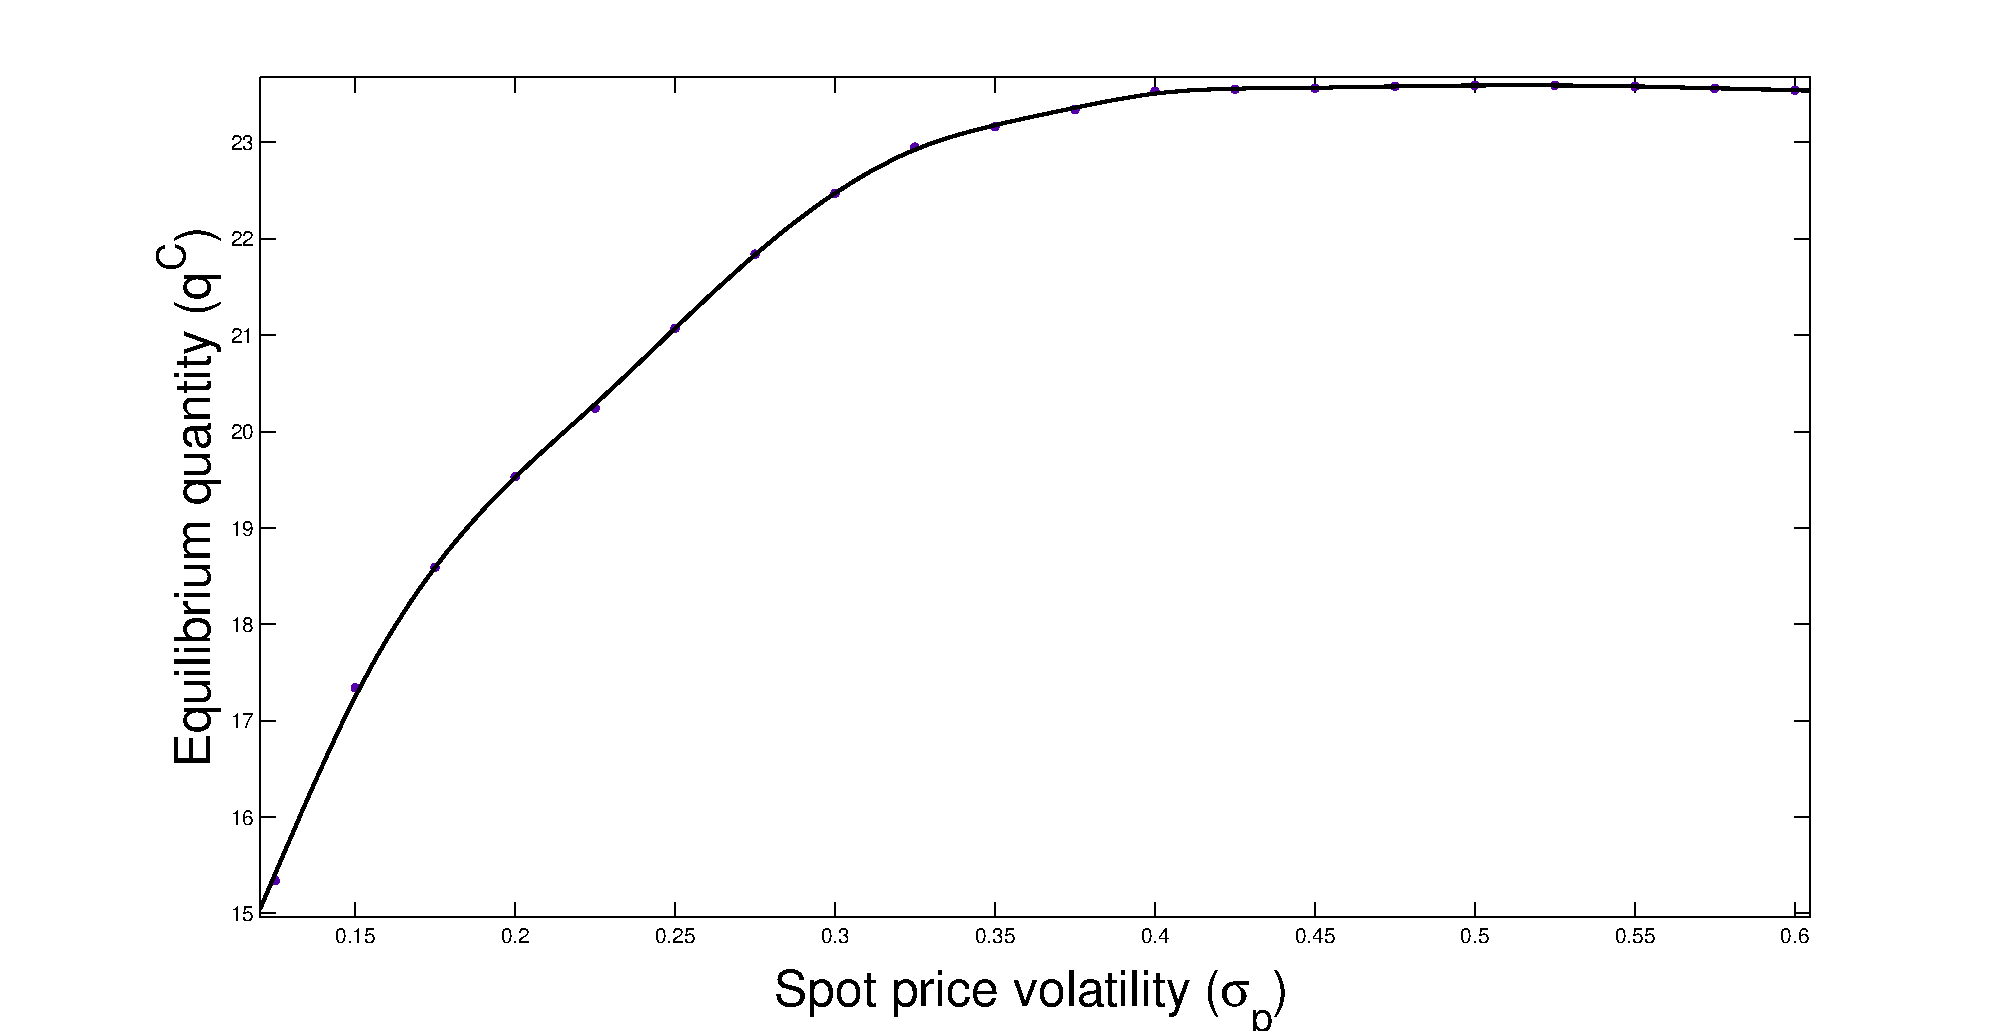
\includegraphics[height=3in]{figures/q_price_vol.pdf}
		\caption{$q_C$ vs $p_\sigma$} \label{qcpvol}
	\end{center}
\end{figure}

\begin{comment}
\subsection{A Real World Example}

We illustrate our model by examining a CFD wind hedge contract between Noble Environmental Power 2008 Hold Co., LLC and Citigroup Energy Inc. The contract is a Fixed-for-Floating financial swap of energy, financially settled against a floating price. The capacity being hedged is the aggregate of 3 wind farms operated by Noble at Altona, Chateaugay and Wethersfiled in the state of New York. The contract term is 10 years, starting April 31, 2009. The settlement period is monthly, and the settlement price is calculated as the weighted average of the day-ahead zonal locational marginal prices (LMPs), with the production levels at the individual wind farms acting as the weights. The strike price is set at 63.05 \$/MWhr and the quantity is set at the P95 level.

Electricity prices were forecast using day-ahead zonal LMP data obtained from the New York Independent System Operator (NYISO) [link]. Wind-farm output was forecast using the National Renewable Energy Laboratory (NREL) [link] wind integration datasets. Forecasting was done by modelling both wind and price as mean-reverting Ornstein-Uhlenbeck processes. Parameter estimation was done using maximum likelihood estimation along with a jack-knife technique [reference].

The forecasted data was used to resolve the model parameters for [equation number]. The resulting optimization problem was then solved using the global optimization solver BARON [reference] on the NEOS [link] server. Since the individual risk aversion factors for the two parties are unknown we perform a comparative statics analysis for the two risk aversion factors. The results are given in Figures \ref{pckb1} through \ref{qc_vs_ks1}.
\begin{figure}[t]
\begin{center}
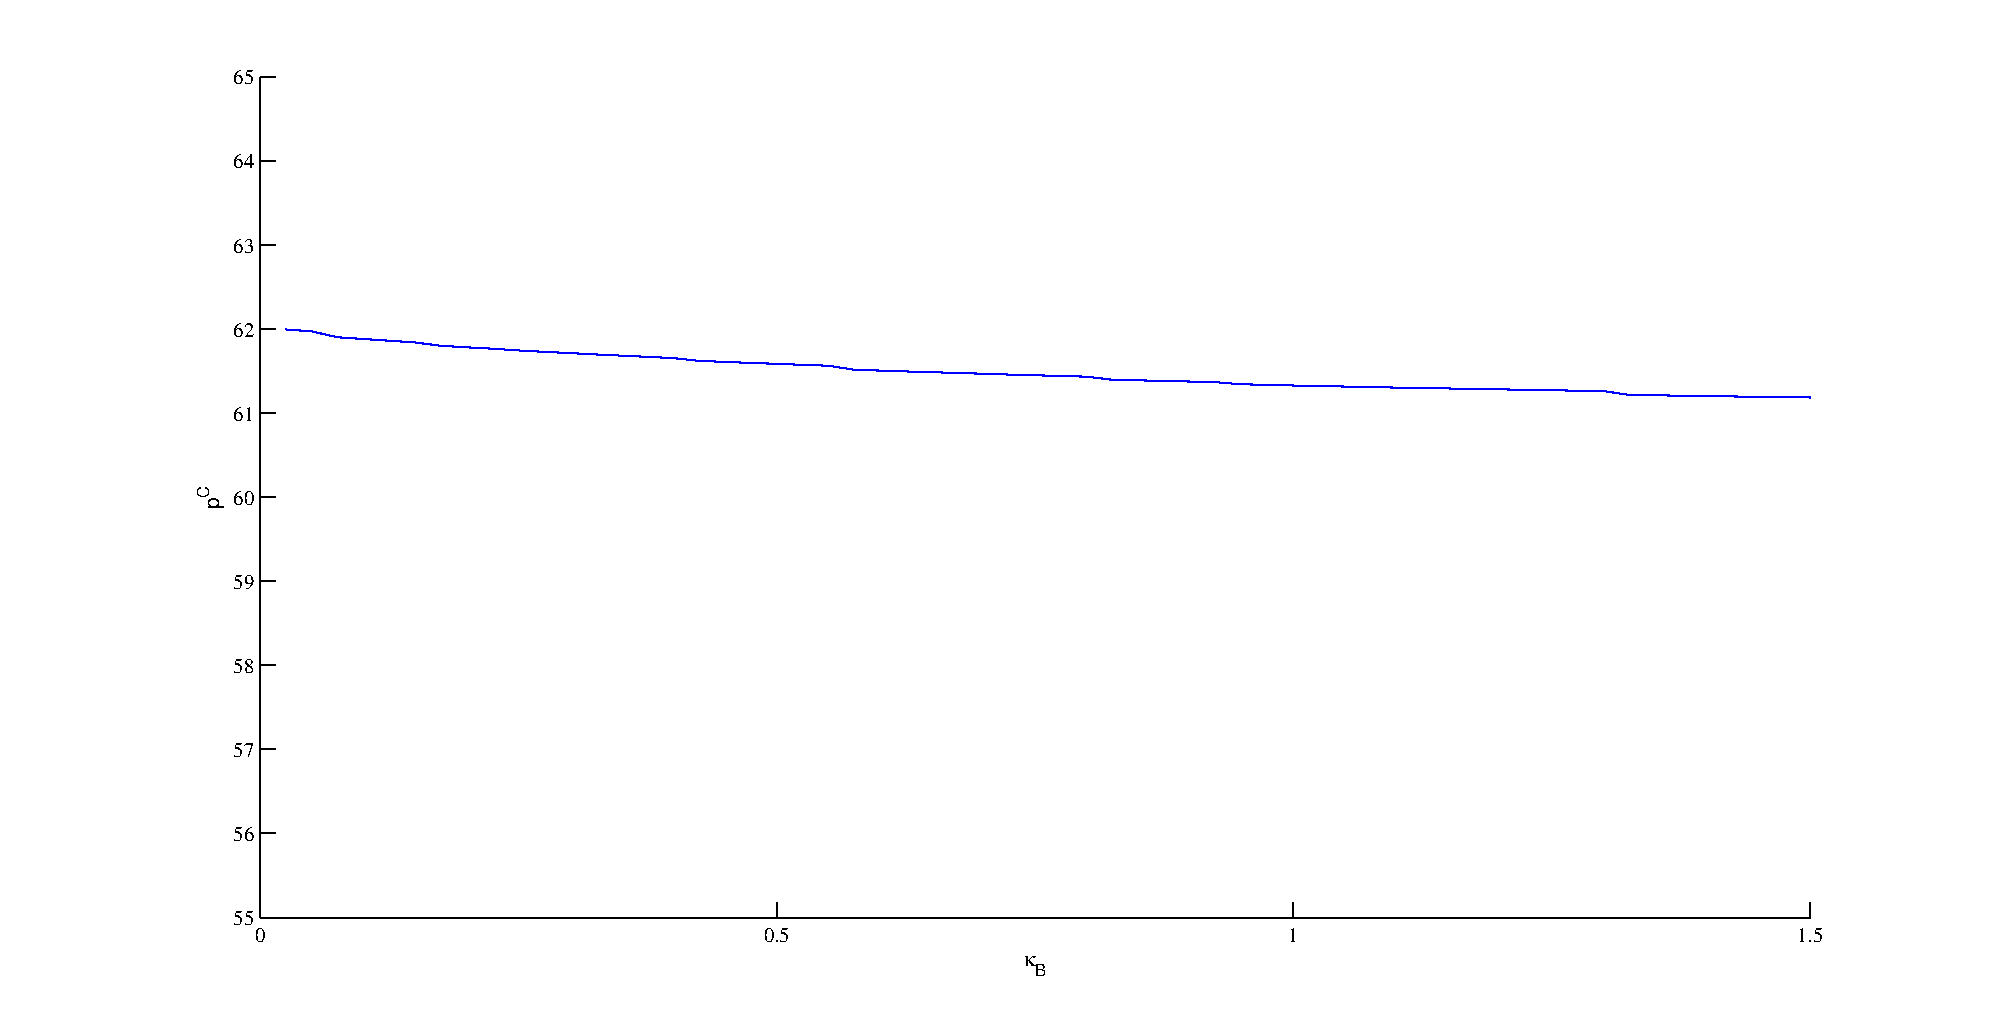
\includegraphics[height=3in]{figures/noble_p_kb.pdf}
\caption{$p_C$ vs $\kappa^B$} \label{pckb1}
\end{center}
\end{figure}
\begin{figure}[t]
\begin{center}
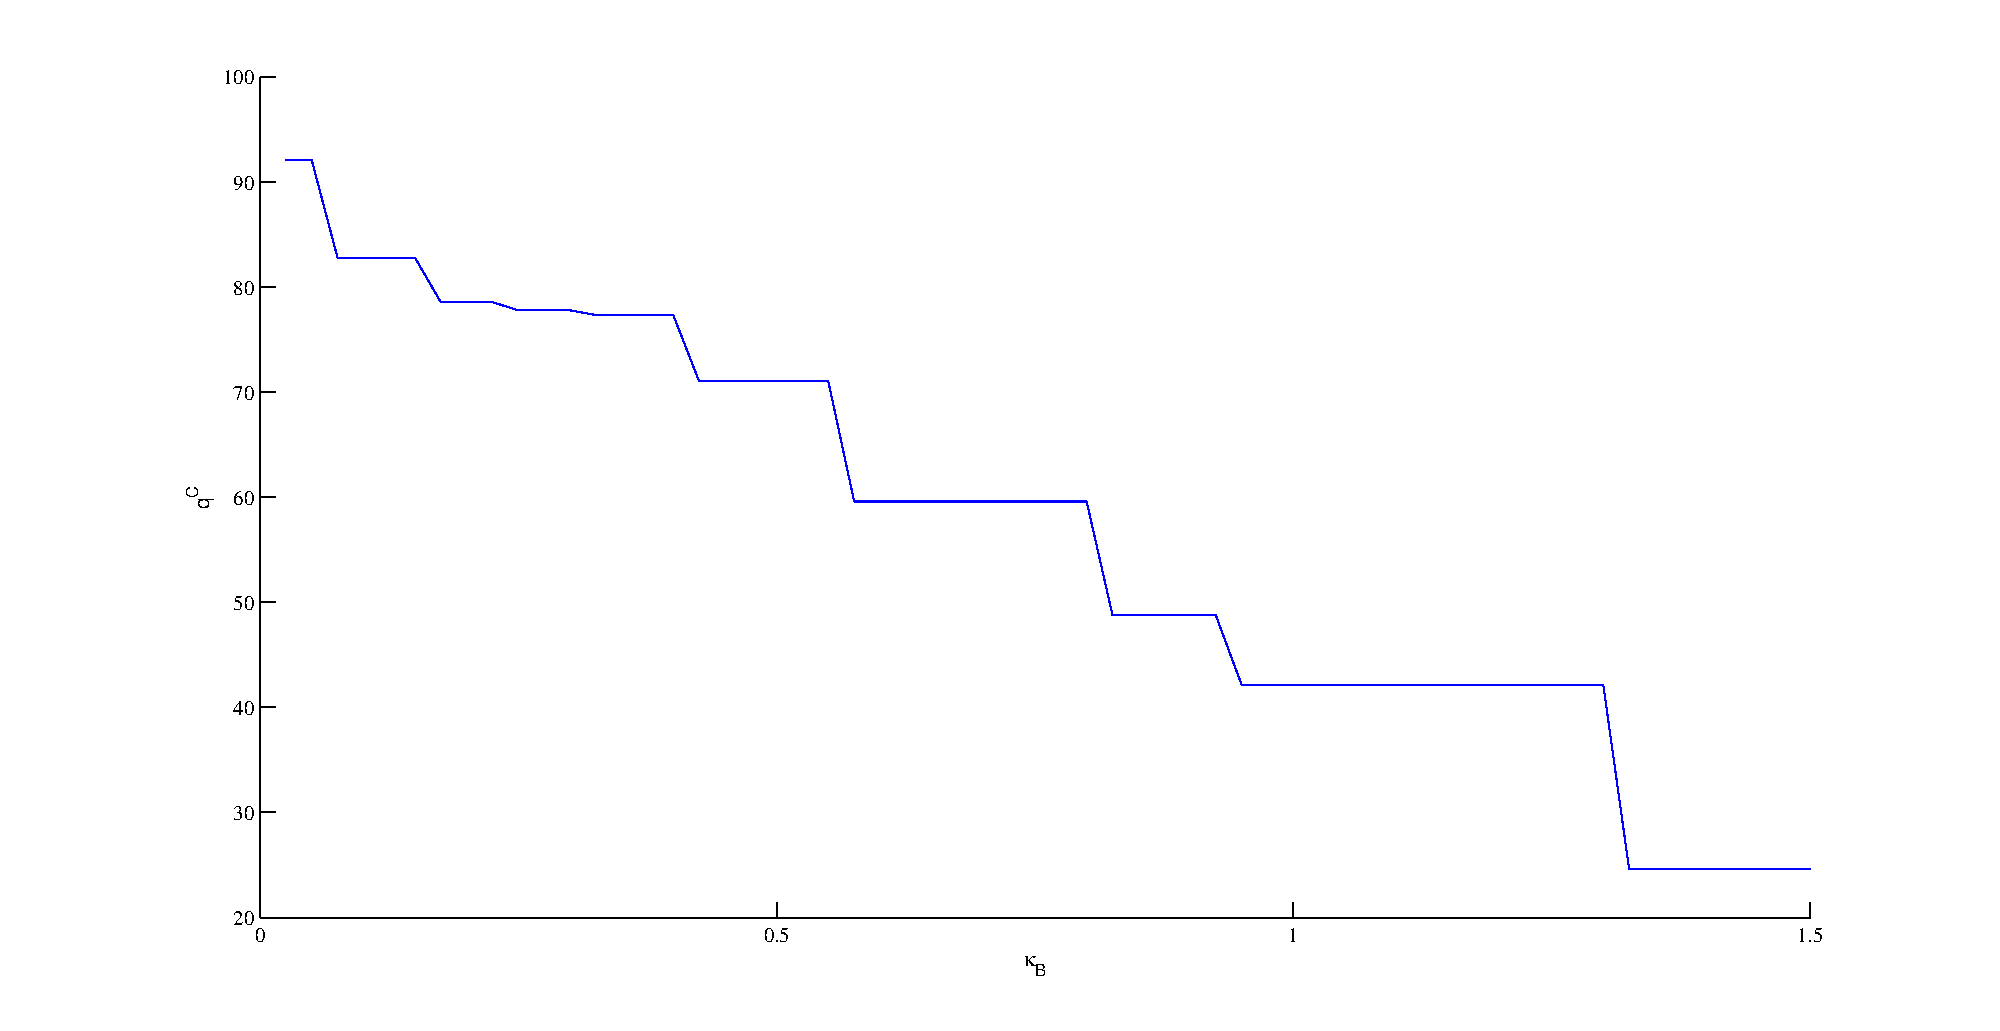
\includegraphics[height=3in]{figures/noble_q_kb.pdf}
\caption{$q_C$ vs $\kappa^B$} \label{qckb1}
\end{center}
\end{figure}
In Figures \ref{pckb1} and \ref{qckb1}, we see the comparative statics for the equilibrium price and quantity with varying risk aversion factors for the buyer. The trends in both price and quantity follow the those we saw in our simulations, although in this case the equilibrium price remains relatively constant. (Insert explanation for the risks and riskb pairs that give price and quantity results near the actual real values and explain the possible deviations).

We also perform comparative statics with respect to the risk aversion factor for the seller. These results are given in Figures \ref{pcks1} and \ref{qcks1}.

\begin{figure}[t]
\begin{center}
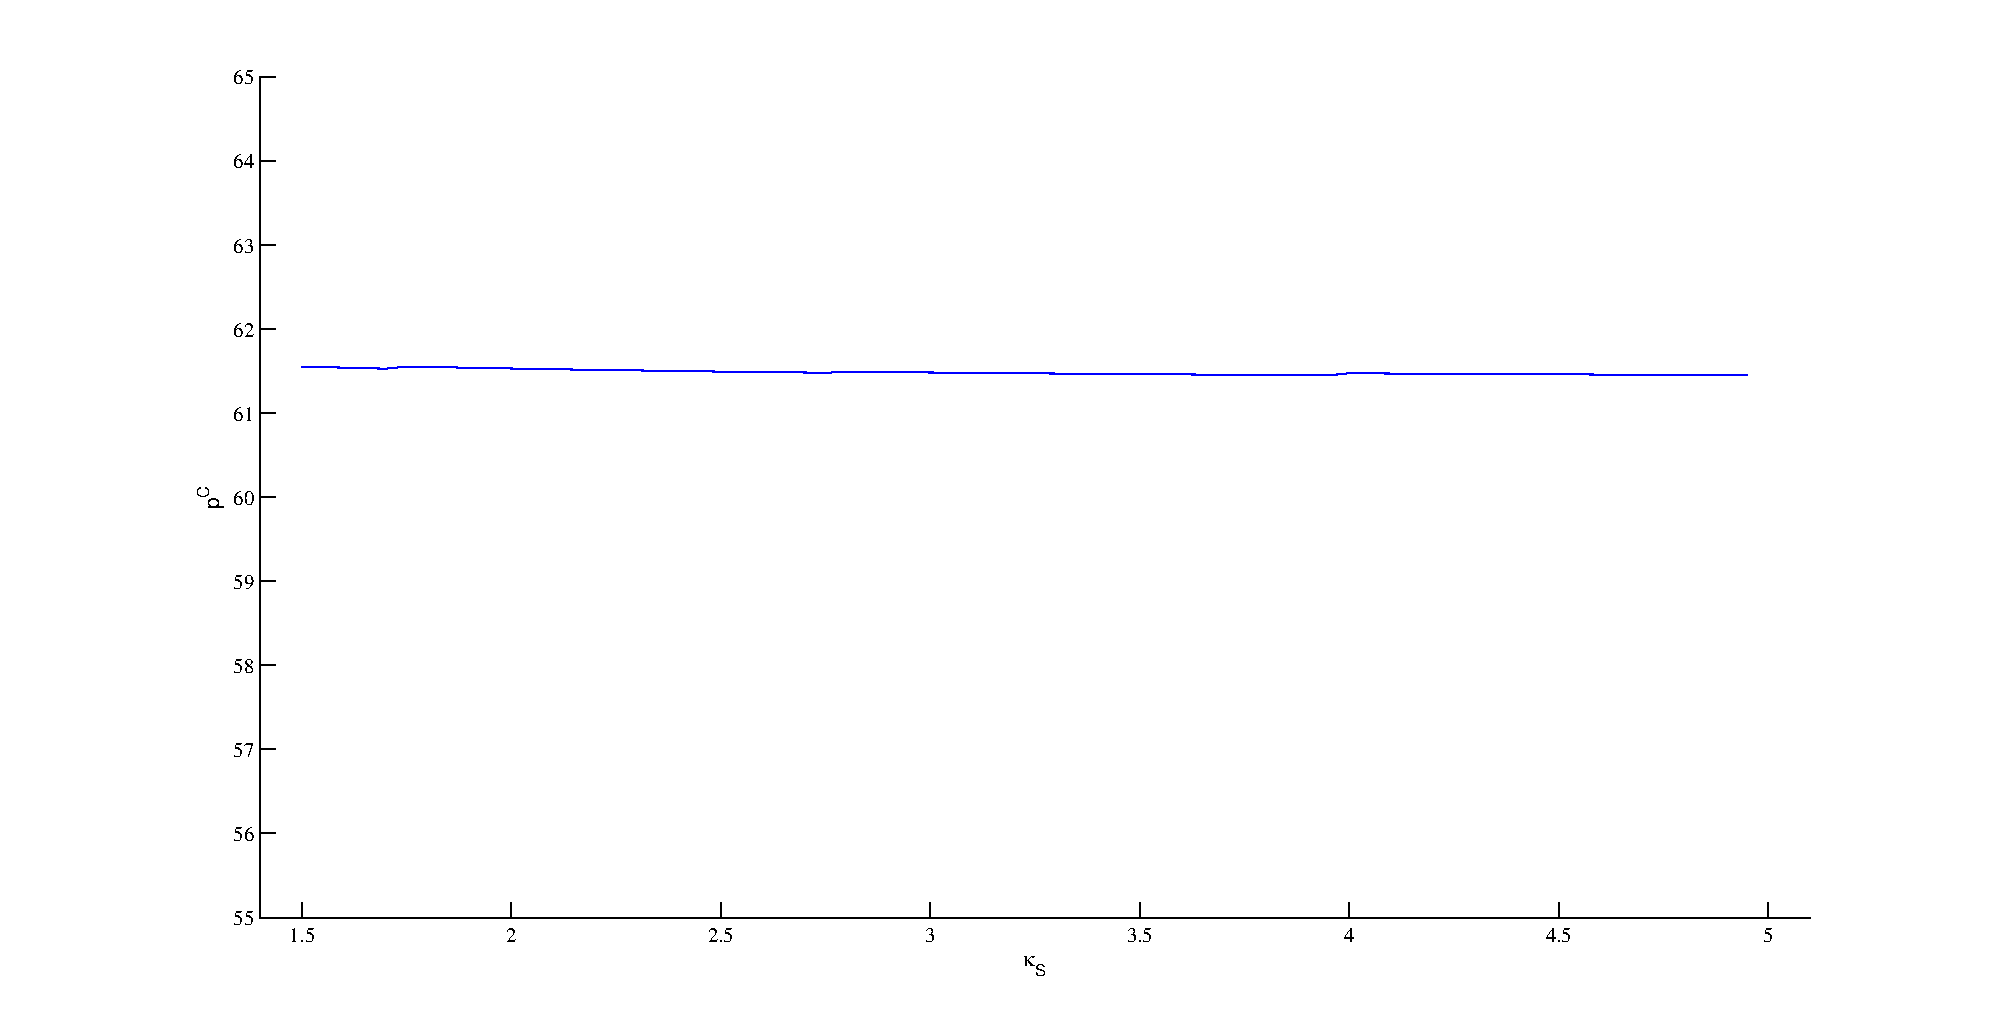
\includegraphics[height=3in]{figures/noble_p_ks.pdf}
\caption{$p_C$ vs $\kappa^S$} \label{pcks1}
\end{center}
\end{figure}
\begin{figure}[t]
\begin{center}
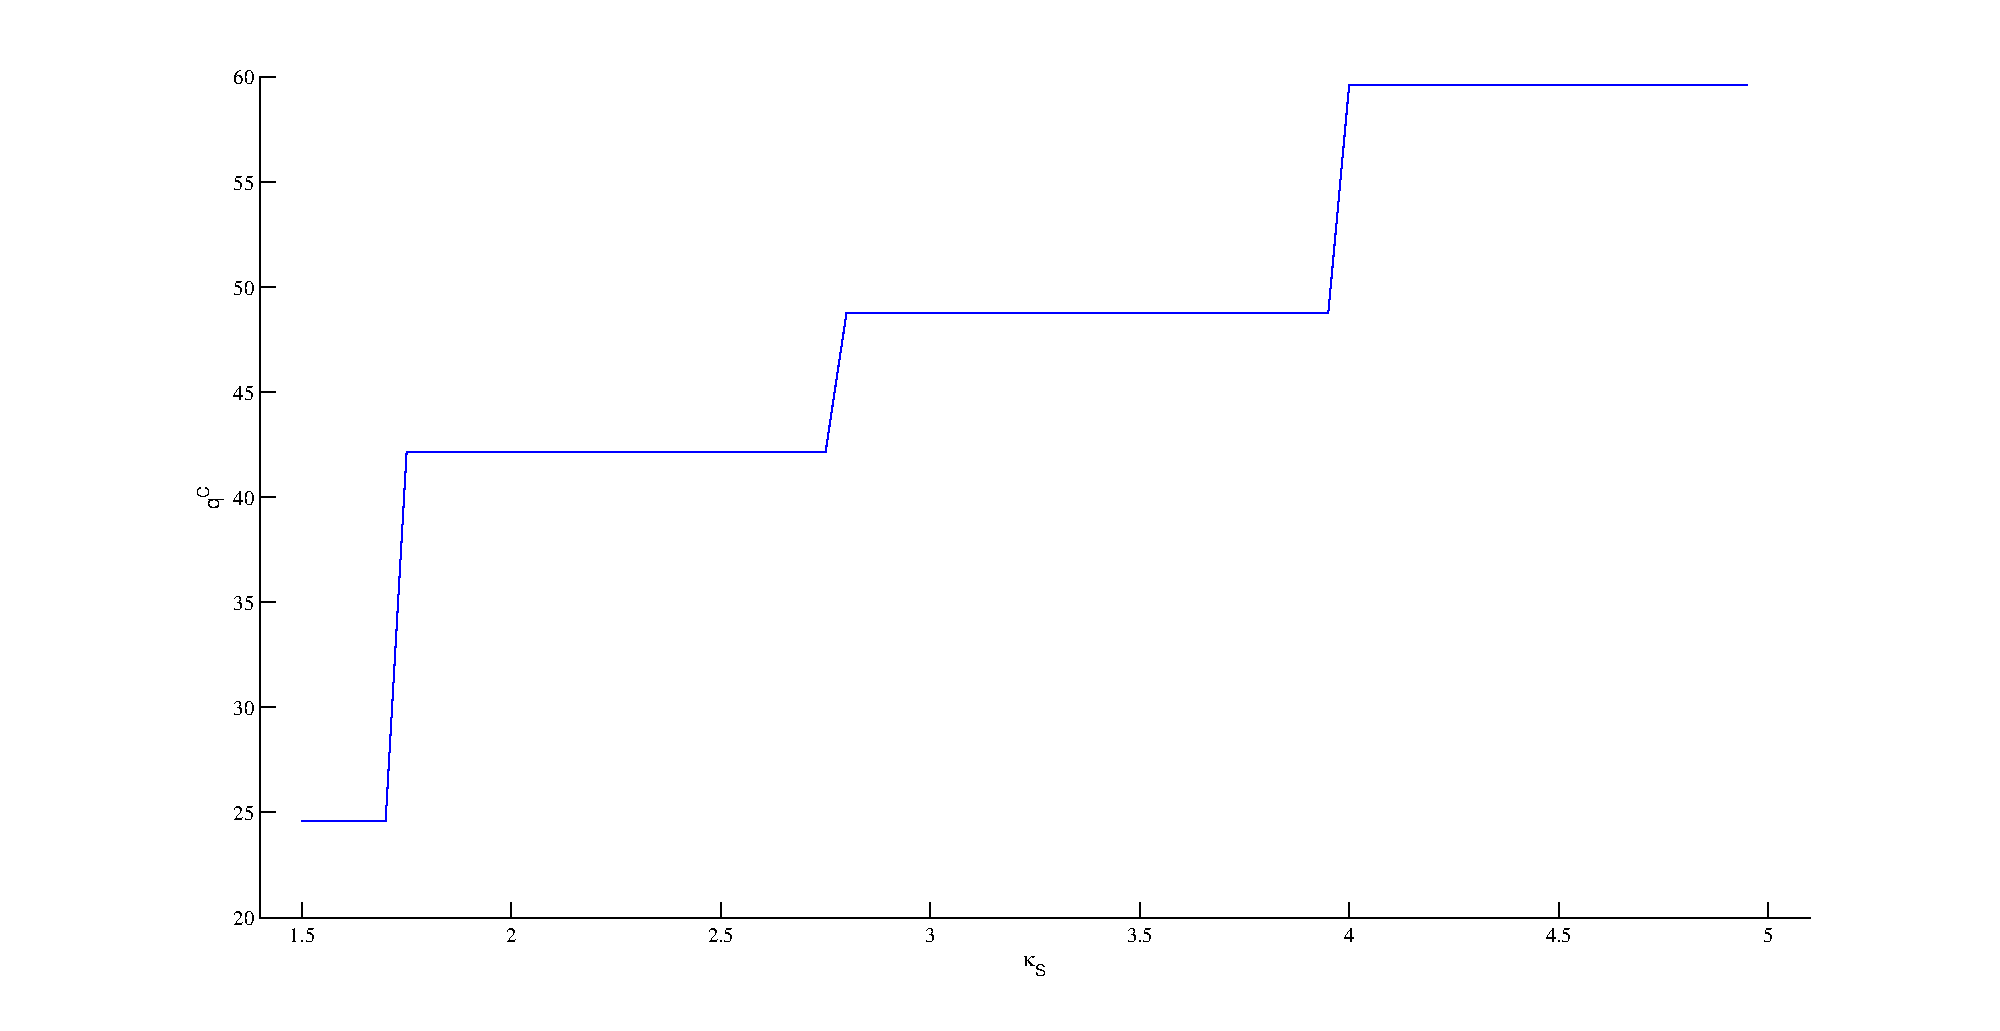
\includegraphics[height=3in]{figures/noble_q_ks.pdf}
\caption{$q_C$ vs $\kappa^S$} \label{qcks1}
\end{center}
\end{figure}

\end{comment}

\section{Conclusion}

The main goal of this paper was to construct a modeling framework for analyzing
the risk transfer aspects of long-term wind hedges between merchant wind
developers and counter-parties. We utilize Nash bargaining theory to model the
negotiation process for the hedging contracts. The risk preferences of the
parties involved are captured using Conditional Cash-Flow at Risk. 

We show that the equilibrium price and quantity for the hedge can be computed by
solving a bilinear stochastic programming problem with expected value
constraints. Since the analytical form for the expectation functions in this
problem is not easily obtainable, we present a sampling scheme to solve the Nash
bargaining optimization problem. Conditions required to ensure consistency of
solutions for the SAA scheme are verified and a validation scheme for
guaranteeing solution quality is outlined.

The Nash bargaining model and the SAA scheme to solve the resulting problem is
then utilized to conduct some numerical experiments. Using a controlled
geometric Brownian motion model to generate the underlying random data, several
problem instances are solved. We also present comparative
statics for the hedge, as input parameters such as the risk attitudes of the
parties involved or market parameters such as price volatility is varied. 

Although commercial global optimization solvers such as BARON were used to solve
the SAA subproblems, we note that these problems have bilinear constraints. This
structure may be exploited to design efficient, globally convergent algorithms.
Since our focus in this paper was on the model and not on computational
efficiency for the solution scheme, we leave a discussion of such algorithms to
future work.

The analytical model we present may be extended to more general hedges in the wind
industry. For instance, quite often wind hedge contracts involve the transfer of
Renewable Energy Certificates (RECs). Such transactions can easily be handled
with minor modification to the NBS optimization problem. Our model can also be
generalized beyond CFD type hedges to other contract structures such as load
following contracts or block power contracts.

This paper mainly considers market risks in the form of spot price variations
and physical risks such as wind speed variation. The scope of the model can also
be broadened by considering other sources of risk, such as credit risk and
liquidity risk. Such an extension would be especially important in the case
where the counter-parties are large organizations, with complex risk management
programs.


\begin{acknowledgements}
%If you'd like to thank anyone, place your comments here
%and remove the percent signs.
\end{acknowledgements}

% BibTeX users please use one of
%\bibliographystyle{spbasic}      % basic style, author-year citations
\bibliographystyle{spmpsci}      % mathematics and physical sciences
%\bibliographystyle{spphys}       % APS-like style for physics
\bibliography{windhedge}   % name your BibTeX data base


\end{document}
% end of file template.tex

